\documentclass[11pt]{amsart}
\linespread{1.25}
\usepackage[margin=3.5cm]{geometry}

\usepackage[english]{babel}
\usepackage{appendix}
\usepackage{amsmath}
\usepackage{amsfonts}
\usepackage{amssymb}
%\usepackage{showlabels}
\usepackage{hyperref}
\usepackage{amsthm}
\usepackage{marginnote}
\usepackage{stmaryrd}
\usepackage{enumitem}
\usepackage[english]{babel}
\usepackage{yfonts}
\usepackage[T1]{fontenc}
\usepackage[utf8x]{inputenc}

\usepackage{calrsfs}
\DeclareMathAlphabet{\pazocal}{OMS}{zplm}{m}{n}

\usepackage{verbatim}
\usepackage{graphicx}
\usepackage{verbatim}
\usepackage{faktor}
\usepackage{xcolor}
\usepackage{xfrac}
\usepackage{tikz,tikz-cd}
\usetikzlibrary{decorations.pathmorphing,decorations.pathreplacing,patterns}

\usepackage[all]{xy}
\usepackage{bbm}
\usepackage{tabularx}
\usepackage{longtable}
\usepackage{tabu}
\usepackage{booktabs}
\usepackage{mathtools}

\usepackage[]{textcomp}
\usepackage[sups]{Baskervaldx}
\usepackage{cabin}
\usepackage[varqu,varl]{inconsolata}
\usepackage[baskervaldx,bigdelims,vvarbb]{newtxmath}
\usepackage[cal=cm]{mathalfa}


\newcommand{\plC}{\scalebox{0.8}[1.3]{$\sqsubset$}}
\newcommand{\sidenote}[1]{\marginpar{\textbf{\color{red}#1}}}

% FIGURES FOR USE LATER
%%%%%%%%%%%%%%%%%%%%%%%%%%%%%%%%%%%%%%%%%%%%%%%%%%%%%%%%%%%%
\def\Yagraph{\tikz[baseline=-3pt,scale=.8]{
\draw (2,0) -- (0,1) (2,0) -- (0,.5) (2,0) -- (0,-1);
\draw (2,0) circle(2pt)[fill=black];
\draw [->] (2,0) -- (2.7,0);
\draw (2.6,0) node[right]{\tiny{$x_k$}};
\draw (0,1) circle(2pt)[fill=white];
\draw (0,.5) circle(2pt)[fill=black];
\draw (0,-.25) node{$\vdots$};
\draw (0,-1) circle(2pt)[fill=black];
\draw [red,fill=red] (0,-2) circle[radius=2pt];
\draw [->,red,thick] (0,-2) -- (2,-2);
\draw (2,-2) node[right,red]{\tiny{$\Sigma(\PP^N|H)$}};
\draw [->,red] (1,-0.9) -- (1,-1.6);

\draw (2.05,0) node[above]{\tiny{$\sqC_0$}};
\draw (0,1) node[left]{\tiny{$\sqC_1$}};
\draw (0,.5) node[left]{\tiny{$\sqC_2$}};
\draw (0,-1) node[left]{\tiny{$\sqC_r$}};
}}

\def\Ybgraph{\tikz[baseline=-3pt,scale=.8]{
\draw (2,0) to[out=120,in=0] (0,1) (2,0) -- (0,1) (2,0) -- (0,.5) (2,0) -- (0,-1);
\draw (2,0) circle(2pt)[fill=black];
\draw [->] (2,0) -- (2.7,0);
\draw (2.6,0) node[right]{\tiny{$x_k$}};
\draw (0,1) circle(2pt)[fill=black];
\draw (0,.5) circle(2pt)[fill=black];
\draw (0,-.25) node{$\vdots$};
\draw (0,-1) circle(2pt)[fill=black];
\draw [red,fill=red] (0,-2) circle[radius=2pt];
\draw [->,red,thick] (0,-2) -- (2,-2);
\draw (2,-2) node[right,red]{\tiny{$\Sigma(\PP^N|H)$}};
\draw [->,red] (1,-0.9) -- (1,-1.6);

\draw (2.05,0) node[above]{\tiny{$\sqC_0$}};
\draw (0,1) node[left]{\tiny{$\sqC_1$}};
\draw (0,.5) node[left]{\tiny{$\sqC_3$}};
\draw (0,-1) node[left]{\tiny{$\sqC_r$}};
}}

\def\Ycgraph{\tikz[baseline=-3pt,scale=.8]{
\draw (2,0) -- (0,1) (2,0) -- (0,.5) (2,0) -- (0,-1);
\draw [->] (2,0) -- (2.7,0);
\draw (2.6,0) node[right]{\tiny{$x_k$}};
\draw (2,0) circle(2pt)[fill=white];
\draw (0,1) circle(2pt)[fill=black];
\draw (0,.5) circle(2pt)[fill=black];
\draw (0,-.25) node{$\vdots$};
\draw (0,-1) circle(2pt)[fill=black];
\draw [red,fill=red] (0,-2) circle[radius=2pt];
\draw [->,red,thick] (0,-2) -- (2,-2);
\draw (2,-2) node[right,red]{\tiny{$\Sigma(\PP^N|H)$}};
\draw [->,red] (1,-0.9) -- (1,-1.6);

\draw (2.05,0) node[above]{\tiny{$\sqC_0$}};
\draw (0,1) node[left]{\tiny{$\sqC_1$}};
\draw (0,.5) node[left]{\tiny{$\sqC_2$}};
\draw (0,-1) node[left]{\tiny{$\sqC_r$}};
}}
%%%%%%%%%%%%%%%%%%%%%%%%%%%%%%%%%%%%%%%%%%%%%%%%%%%%%%%%%%%%%%

\newcommand{\mathsq}[1]{#1}

\newcommand{\sqC}{\scalebox{0.8}[1.3]{$\sqsubset$}}

\newcommand{\pM}{\pazocal{M}}
\newcommand{\TT}{\operatorname{T}}
\newcommand{\oM}{\overline{\mathcal{M}}}
\newcommand{\M}[4]{\overline{\mathcal{M}}_{#1,#2}(#3,#4)}

\newcommand{\Mlog}[4]{\overline{\mathcal{M}}^{\operatorname{log}}_{#1,#2}(#3,#4)}
\newcommand{\MLog}{\overline{\mathcal{M}}^{\operatorname{log}}}
\newcommand{\Mpunct}[4]{\overline{\mathcal{M}}^{\operatorname{punct}}_{#1,#2}(#3,#4)}
\newcommand{\MG}[4]{\overline{\mathcal{M}}^{\rm G}_{#1,#2}(#3,#4)}
\newcommand{\Q}[4]{\mathcal{Q}_{#1,#2}(#3,#4)}
\newcommand{\Qe}[4]{\mathcal{Q}^{\epsilon}_{#1,#2}(#3,#4)}
\newcommand{\Qt}[4]{\widetilde{\mathcal Q}_{#1,#2}(#3,#4)}
\newcommand{\QG}[4]{\mathcal{Q}G_{#1,#2}(#3,#4)}
\newcommand{\QGe}[4]{\mathcal{Q}G^{\epsilon}_{#1,#2}(#3,#4)}
\newcommand{\D}[3]{\mathcal{D^Q}(#1,#2,#3)}
\newcommand{\E}[3]{\mathcal{E^Q}(#1,#2,#3)}
\newcommand{\PP}{\mathbb P}
\newcommand{\Z}{\mathbb{Z}}
\newcommand{\VZ}{\pazocal{V\!Z}}
\newcommand{\tVZc}[4]{\widetilde{\mathcal{V\!Z}}^{\rm{ctr}}_{#1,#2}(#3,#4)}
\newcommand{\VZc}[4]{\mathcal{V\!Z}_{#1,#2}(#3,#4)}
\newcommand{\VZcLi}[4]{\mathcal{V\!Z}^{\rm{ctr, Li}}_{#1,#2}(#3,#4)}
\newcommand{\VZrel}[4]{\mathcal{V\!Z}^{\rm{rel}}_{#1,#2}(#3,#4)}
\newcommand{\stab}{\rm{stab}}
\newcommand{\st}{\star}
\newcommand{\stC}{C'}
\newcommand{\stpi}{\pi'}
\newcommand{\sts}{s'}
\newcommand{\N}{\mathbb{N}}
\newcommand{\OO}{\mathcal{O}}
\renewcommand{\to}{\rightarrow}
\newcommand{\A}{\mathcal A}
\newcommand{\B}{\mathcal B}
\newcommand{\C}{\mathfrak C}
\newcommand{\cC}{\mathcal C}
\newcommand{\EE}{\mathbf{E}}
\renewcommand{\L}{\mathcal L}
\newcommand{\LL}{\mathbf{L}}
\newcommand{\MM}{\mathfrak M}
\newcommand{\Aaff}{\mathbb{A}}
\newcommand{\kfield}{\Bbbk}
\newcommand{\comp}{\chi}
\newcommand{\sst}{\sigma^{\operatorname{ss}}}
\newcommand{\Pic}{\operatorname{Pic}}
\newcommand{\Def}{\operatorname{Def}}
\newcommand{\Spec}{\operatorname{Spec}}
\newcommand{\Proj}{\operatorname{Proj}}
\newcommand{\Hom}{\operatorname{Hom}}
\newcommand{\Ext}{\operatorname{Ext}}
\newcommand{\Gm}{\mathbb{G}_{\text{m}}}
\newcommand{\virt}[1]{[#1]^{\operatorname{virt}}}
\newcommand{\vip}[1]{[#1]^{\operatorname{prod}}}
\newcommand{\Id}{\operatorname{Id}}
\newcommand{\CC}{\mathbb{C}}
\newcommand{\QQ}{\mathbb{Q}}
\newcommand{\HH}{\operatorname{H}}
\newcommand{\Achow}{\operatorname{A}}
\newcommand{\pt}{\operatorname{pt}}
\newcommand{\bq}{\begin{equation}}
\newcommand{\eq}{\end{equation}}
\newcommand{\ba}{\begin{aligned}}
\newcommand{\ea}{\end{aligned}}
\newcommand{\be}{\begin{enumerate}}
\newcommand{\ee}{\end{enumerate}}
\newcommand{\bsm}{\left(\begin{smallmatrix}}
\newcommand{\esm}{\end{smallmatrix}\right)}                   
\newcommand{\bpm}{\begin{pmatrix}}
\newcommand{\epm}{\end{pmatrix}}
\newcommand{\barr}{\begin{displaymath}\begin{array}{cccc}}
\newcommand{\earr}{\end{array}\end{displaymath}}
\newcommand{\barrl}{\begin{displaymath}\begin{array}{lcl}}
\newcommand{\earrl}{\end{array}\end{displaymath}}
\newcommand{\barl}{\begin{displaymath}\begin{array}{l}}
\newcommand{\earl}{\end{array}\end{displaymath}}
\newcommand{\bxym}{ \begin{displaymath}\xymatrix }
\newcommand{\exym}{\end{displaymath}}
\newcommand{\bcd}{\begin{center}\begin{tikzcd}}
\newcommand{\ecd}{\end{tikzcd}\end{center}}
\newcommand{\R}{\operatorname{R}^{\bullet}}
\newcommand{\dvr}{\Delta}
%\newcommand{\sslash}{\mathbin{/\mkern-6mu/}}
\newcommand{\tr}{{\rm tr}}
\newcommand{\Isom}{\text{Isom}}
\newcommand{\pr}{\operatorname{pr}}
\newcommand{\ev}{\operatorname{ev}}
\newcommand{\fgt}{\operatorname{fgt}}
\newcommand{\codim}{\operatorname{codim}}
\newcommand{\vdim}{\operatorname{vdim}}
\newcommand{\ildef}[1]{\emph{#1}}
\newcommand{\om}[1]{\mathcal{#1}}
\newcommand{\h}{\operatorname{h}}
\newcommand{\Aut}{\operatorname{Aut}}
\newcommand{\Acal}{\mathcal{A}}
\newcommand{\Scal}{\mathcal{S}}
\newcommand{\Mcal}{\mathcal{M}}
\newcommand{\Dcal}{\mathcal{D}}
\newcommand{\Ncal}{\mathcal{N}}
\newcommand{\Lcal}{\mathcal{L}}
\newcommand{\Ccal}{\mathcal{C}}
\newcommand{\Pcal}{\mathcal{P}}
\newcommand{\Ycal}{\mathcal{Y}}
\newcommand{\cchern}{\mathrm{c}}
\newcommand{\ol}[1]{\overline{#1}}
\newcommand{\ul}[1]{\underline{#1}}
\newcommand{\op}[1]{\operatorname{#1}}
\newcommand{\gp}{\operatorname{gp}}
\newcommand{\RR}{\mathbb{R}}
\newcommand{\NN}{\mathbb{N}}
\newcommand{\ovm}[1]{\overline{\mathcal{#1}}}
\newcommand{\ovt}[1]{\widetilde{\mathcal{#1}}}
\newcommand{\ov}[1]{\overline{#1}}

\theoremstyle{definition}
\newtheorem{thm}{Theorem}[section]
\newtheorem{lem}[thm]{Lemma}
\newtheorem{lemma}[thm]{Lemma}
\newtheorem{prop}[thm]{Proposition}
\newtheorem{cor}[thm]{Corollary}
\newtheorem*{teo*}{Theorem}
\newtheorem{ipotesi}{ipotesi}
\newtheorem*{nota}{Nota}
\newtheorem{claim}{Claim}
\newtheorem{question}[thm]{Question}
\newtheorem{conj}[thm]{Conjecture}

\newtheorem{innercustomthm}{Theorem}
\newenvironment{customthm}[1]
  {\renewcommand\theinnercustomthm{#1}\innercustomthm}
  {\endinnercustomthm}

\theoremstyle{definition}
\newtheorem{example}[thm]{Example}
\newtheorem{ex}[thm]{Example}
\newtheorem{dfn}[thm]{Definition}
\newtheorem{definition}[thm]{Definition}
\newtheorem{aside}[thm]{Aside}
\newtheorem{remark}[thm]{Remark}
\newtheorem{com}[thm]{Comment}
\newtheorem{num}{Number}
\newtheorem*{sketch}{Sketch}
\newtheorem*{rem}{Remark}
\newtheorem*{aside*}{Aside}
\newtheorem*{acknowledgements}{Acknowledgements}

\newlist{steps}{enumerate}{1}
\setlist[steps, 1]{label = Step (\arabic*):}

\newcommand{\ilemph}[1]{\emph{#1}}

\setcounter{tocdepth}{2}

\newcommand{\todo}[1]{\vspace{5mm}\par \noindent
\framebox{\begin{minipage}[c]{0.95 \textwidth} \tt #1\end{minipage}} \vspace{5mm} \par}

\def\ti{-\allowhyphens}
\newcommand{\thismonth}{\ifcase\month % case 0 --- impossible!
  \or January\or February\or March\or April\or May\or June%
  \or July\or August\or September\or October\or November%
  \or December\fi}
\newcommand{\thismonthyear}{{\thismonth} {\number\year}}
\newcommand{\thisdaymonthyear}{{\number\day} {\thismonth} {\number\year}}

\title{Gromov--Witten theory of hypersurfaces in genus one}
\author{Luca Battistella, Navid Nabijou and Dhruv Ranganathan}
\date{\thismonthyear}

\begin{document}


\begin{abstract}
\end{abstract}

\maketitle

\appendixtitletocoff
\tableofcontents

\newpage


\subsection{Recursion procedure for reduced rubber integrals} In the recursion above, certain terms appear which are integrals over moduli spaces of reduced log stable maps to rubber (as defined in \S \ref{}):
\begin{equation*}\VZ_{1,\alpha}(P|H_0+H_\infty)_{\Gm}.\end{equation*}
In this section we provide a recursive algorithm for computing such integrals. For convenience we denote the \textbf{horizontal degree} of the rubber map by:
\begin{equation*} d := \sum_{i=1}^n \alpha_i .\end{equation*}
Recall that the $\alpha_i$ may be positive or negative (recording tangencies with respect to $H_\infty$ and $H_0$, respectively) and that $d \geq 0$ always. First suppose that $d=0$. Then the usual rubber moduli space decomposes as
\begin{equation*} \MLog_{1,\alpha}(P|H_0 + H_\infty)_{\Gm} = \MLog_{1,\alpha}(\PP^1|0+\infty)_{\Gm} \times H \end{equation*}
and the first term on the right-hand side is birational to the double ramification locus in $\ol\Mcal_{1,n}$. This locus has a main component (the closure of the locus of smooth curves) and one other ``exceptional'' component, consisting of split curves where all the markings belong to the rational tail. The corresponding reduced rubber space is birational to the main component, and thus we can identify its class by subtracting off the class of the exceptional component. This gives
\begin{equation*} \pi_\st [\VZ_{1,\alpha}(P|H_0+H_\infty)_{\Gm}] = \left( [\ol\Mcal_{1,n}^\alpha] - [D] \right) \times [H] \in \Achow_\st ( \ol\Mcal_{1,n} \times H ) = \Achow_\st ( \ol\Mcal_{1,n}(H,0) ) \end{equation*}
where $\pi \colon \VZ_{1,\alpha}(P|H_0+H_\infty)_{\Gm} \to \ol\Mcal_{1,n}(H,0)$ is the map which forgets the log structure and collapses the map, $D$ is the boundary locus of split curves described above, and $[\ol\Mcal_{1,n}^\alpha]$ is the classical double ramification cycle, which has an explicit formula in terms of tautological classes \cite{Hain,JPPZ}. This allows us to compute the integral over the rubber space as a tautological integral on the moduli space of curves.

Now suppose that $d>0$. If there is a marking $x_k$ which carries no insertion and has $\alpha_k \neq 0$, then consider the morphism which forgets $x_k$ and collapses the map:
\begin{equation*} \VZ_{1,\alpha}(P|H_0+H_\infty)_{\Gm} \xrightarrow{\pi} \VZ_{1,n-1}(H,d). \end{equation*}
These moduli spaces are log smooth and of the same dimension. Over the nice locus in $\VZ_{1,n-1}(H,d)$, $\pi$ has degree $\alpha_k^2$, arising from a choice of $\alpha_k$-torsion point on the source elliptic curve. Thus we have:
\begin{equation*} \pi_\st [\VZ_{1,\alpha}(P|H_0+H_\infty)_{\Gm}] = \alpha_k^2\cdot [\VZ_{1,n-1}(H,d)].\end{equation*}
Since all the insertions are pulled back from the right-hand side (up to modifying psi classes by some boundary strata which we can then also compute recursively) we can perform the integral on $\VZ_{1,n-1}(H,d)$ inductively.\footnote{(Navid) Say something here about the degree being smaller}

It remains to deal with the case where all of the relative markings carry insertions. The idea is to reduce to the case above by introducing an additional marking. Note first that every reduced rubber integral which appears in our recursion must either have a marking of negative tangency (i.e. tangent to $H_0$), or a marking with no insertions: indeed, the only boundary locus with no negative-tangency marking occurs when the entire curve is mapped to higher level, in which case (since we are assuming $d>0$) the curve is generically irreducible, and on this curve we have at least one fictitious marking (of positive tangency $1$) with no insertion.

Therefore we may assume that there is at least one point of negative tangency, corresponding to a node at which we will glue. Notice that in our recursion these points only ever carry evaluation classes. Consider the following rubber space of dimension one higher, obtained by introducing an additional non-relative marking:
\begin{equation} \label{bigger rubber space}\VZ_{1,\alpha \cup (0)}(P|H_0+H_\infty)_{\Gm}. \end{equation}
Given a moduli point in this space, consider the piecewise-linear function on the associated tropical moduli space which sends a tropical map to the sum of the target edge lengths. This defines a line bundle and section on the space \eqref{bigger rubber space} which vanishes precisely on the locus where the target splits; moreover the vanishing orders may be read off from the tropical data as in \S \ref{}. It is not hard to see \cite{EKatz} that the first Chern class of the line bundle is
$\Psi_0 + \Psi_\infty$, a sum of target psi classes which may be identified with evaluation and psi classes on the source curve as in \cite[Construction 5.1.17]{GathmannThesis}. 

Now choose a point $x_1$ which carries only evaluation classes, and let $x_0$ denote the new non-relative marking we have introduced. If $\gamma$ was the class we were originally trying to integrate, consider the class $\tilde\gamma$ on \eqref{bigger rubber space} obtained from $\gamma$ by replacing $\ev_1$ by $\ev_0$. We obtain a recursion formula:
\begin{equation*} (\Psi_0+\Psi_\infty)\cdot \tilde\gamma \cap [\VZ_{1,\alpha\cup(0)}(P|H_0+H_\infty)_{\Gm}] = \sum_{\Gamma} m_\Gamma \cdot \tilde\gamma \cap [\ol\Mcal_{\Gamma}]. \end{equation*}
The right-hand side is a sum over irreducible components $\ol\Mcal_\Gamma$ of the locus where the target splits, with multiplicites $m_\Gamma$ calculated from the tropical picture. Each of these components can be written as a fibre product of (reduced) rubber spaces. One of these components is the locus where $x_0$ and $x_1$ belong to a trivial rational bubble:

[FIGURE]

The corresponding moduli space is $\VZ_{1,\alpha}(P|H_0+H_\infty)_{\Gm}$ and we have $\ev_0=\ev_1$ here, so the contribution of this locus is precisely the original rubber integral we were trying to calculate. The remaining terms on the right-hand side have, by design, no insertion at $x_1$ and hence can be computed via the trick described previously. Finally, the left-hand side also has no insertion at $x_1$ and so can be computed by the same method. Here we are assuming that $x_1$ is not the only negative-tangency marking, so that $\Psi_0$ can be interpreted as an insertion on a marking different from $x_1$; if this is not the case, then a similar argument works by splitting $x_1$ into two markings of tangency $(\alpha_1+1,-1)$.

\textbf{What if $\alpha_1=-1$?}

\newpage





If there is a relative marking with no insertion, we can forget that marking and compare to the main component of absolute maps to $H$.

Suppose therefore that every relative marking has insertions. At least one of these must have only evaluation classes (since any of the nodal markings will only have evaluation classes). Fix that one: call it $x$.

Consider the rubber VZ space with one additional marking $x_0$ with contact order zero. On this rubber space, take same as insertions as before, except replace $\ev_x$ with $\ev_{x_0}$.

Consider the locus where the target splits. This can be expressed in terms of tautological classes in several ways (which gives us the left-hand side).

Firstly, by E. Katz's thesis (actually, this is an easy argument using $\MM_{0,2}$ Vakil--Zinger identification of tangent and cotangent spaces on a genus zero curve). We get $\Psi_0 + \Psi_\infty$ (target psi classes).

Alternatively, take the piecewise-linear $\RR_{\geq 0}$-valued function on the tropical moduli space of the VZ rubber space which sends a tropical map to the weighted sum of the edge lengths (weighted by expansion factors). We can see that the Chern class is weighted sum of source psi classes (which agree with the target psi classes by pull-back), and we calculate the vanishing orders by the same locally toric method.

Either way, the left-hand side is determined. Now look at the right-hand side. One component of this is where the $x_0$ and $x$ are contained in a trivial bubble. Therefore $\ev_x = \ev_0$ and we recover the integral we are interested in.

On the other components, the marking $x$ will always be insertion-free; hence we can forget $x$. So we get an integral over main component of maps to $H$. Note that this reduced invariant of $H$ will be of lower degree than the one we set out to compute. So the recursion isn't circular.

\textbf{Addendum} You have to be a bit careful about the target psi class on the larger space. We need to integrate over this, and the standard approach is to identify it with $\alpha_i \psi_i + \ev_i^\st H$ for $x_i$ any marking tangent to the corresponding divisor. Remember we are trying to move all the insertions off $x_k$. If there is some other marking $x_i$ tangent to the same divisor as $x_k$ then we're fine - just interpret the target psi class as an insertion on $x_i$. If not, we're forced to get an insertion at $x_k$ on the larger space, and we're stuck. In this case, we need to modify the recursion scheme slightly: instead of introducing an additional non-relative marking, split $x_k$ into two markings of tangency $1$ and $\alpha_k - 1$ (really, any splitting of $\alpha_k$ will probably do). Then we can safely move all the insertions (including the target psi class) onto one of these, and leave the other free to forget. Note this works even if $\alpha_k=1$.\medskip

\textbf{Note} It might be worth noting that this idea of recursion on rubber spaces by taking $c_1$ of a line bundle appears to have already appeared in E. Katz's paper. Maybe he was right that there's a lot of good stuff there!

\newpage

\subsection{Gathmann's line bundle via tropical geometry} For each marking $x_k$ we consider the locus in $\VZ_{1,\alpha}(\PP^N|H)$ where $x_k$ belongs to an internal component of the collapsed map. We use the log structure on $\VZ_{1,\alpha}(\PP^N|H)$ to construct a line bundle $\Lcal_k$ together with a section $s_k$ vanishing along this locus. We use the correspondence with tropical geometry to identify $\cchern_1(\Lcal_k)$ in terms of tautological classes on $\VZ_{1,\alpha}(\PP^N|H)$, and to compute the vanishing order of $s_k$ along the components of its zero set.

The pair $(\Lcal_k,s_k)$ is most naturally constructed on the moduli space $\MLog_{1,\alpha}(\PP^N|H)$ of non-expanded log maps; the corresponding pair on $\VZ_{1,\alpha}(\PP^N|H)$ will be obtained via pull-back. Consider therefore a moduli point in $\MLog_{1,\alpha}(\PP^N|H)$ and let $Q^\vee_{\RR}$ be the corresponding tropical moduli space (viewed as a rational polyhedral cone). Over this cone we have a universal tropical curve and map
\bcd
\sqC \ar[d,"\pi"] \ar[r,"f"] & \RR_{\geq 0} \\
Q^\vee_{\RR} \ar[u, bend left=40pt, "x_k" left]
\ecd
where $x_k$ is the section which for every point $\lambda \in Q^\vee_{\RR}$ picks out the vertex of $\sqC_\lambda$ containing the leg $x_k$. The composition $f \circ x_k \colon Q^\vee_{\RR} \to \RR_{\geq 0}$ defines a piecewise-linear function on $Q_{\RR}^\vee$ whose preimage over the open cone $\RR_{>0}$ consists of those tropical maps where $x_k$ belongs to an internal component. Dually we obtain an element of the minimal monoid $Q$ at the moduli point, and this globalises to produce a section of the ghost sheaf on $\MLog_{1,\alpha}(\PP^N|H)$. In the usual way this induces a line bundle and section $(\Lcal_k,s_k)$ on the moduli space, and the tropical description above shows that the zero locus of $s_k$ is (set-theoretically) the locus where $x_k$ belongs to an internal component.

We now calculate $\cchern_1(\Lcal_k)$. Choose a family of log stable maps over $S$ and let $\mu \in \Gamma(S,\ol{M}_S)$ be the global section of the ghost sheaf constructed in the previous paragraph. This pulls back along $\pi$ to give a global section $\pi^\flat(\mu) \in \Gamma(C,\ol{M}_C)$.  Interpreted as a piecewise-linear function on the tropicalisation $\sqC$ with values in $\ol{M}_S$ \cite[Remark 7.3]{CavalieriChanUlirschWise}, this assigns $\mu$ to every vertex and has slope zero along every edge. By construction, the line bundle associated to this section is $\pi^\st \Lcal_k$. Consider on the other hand the generator $1 \in \N = \Gamma(\PP^N,\ol{M})$ with associated line bundle $\OO(H)$. The section $f^\flat(1) \in \Gamma(C,\ol{M}_C)$ has associated line bundle $f^\st\OO(H)$. If we let $v$ denote the vertex containing $x_k$, then by construction $f^\flat(1)$ assigns $\mu$ to $v$ and has slope $\alpha_k$ along the leg $x_k$. Thus if we consider the difference $f^\flat(1) - \pi^\flat(\mu)$ then this assigns $0$ to $v$ and still has slope $\alpha_k$ along $x_k$. Thus by \cite[Proposition 2.4.1]{RSPW} the corresponding line bundle restricted to $C_v$ is given by
\begin{equation*} \OO_{C_v} \left(\alpha_k x_k + \sum_e \mu_e x_e \right) \end{equation*}
where the sum is over the edges $e$ adjacent to $v$ and distinct from $x_k$. Thus we see that:
\begin{equation*} \left( f^\st\OO(H) \otimes \pi^\st \Lcal_k^{-1} \right) \big|_{C_v} = \OO_{C_v} \left(\alpha_k x_k + \sum_e \mu_e x_e \right).\end{equation*}
Since $x_k$ factors through $C_v$ we may pull back along $x_k$ to obtain
\begin{equation*} \Lcal_k = x_k^\st\pi^\st \Lcal_k = x_k^\st \OO_{C_k}(-\alpha_k x_k) \otimes x_k^\st f^\st\OO(H) = x_k^\st \OO_{C_k}(-\alpha_k x_k) \otimes \ev_k^\st \OO(H) \end{equation*}
and taking Chern classes gives:
\begin{equation*} \cchern_1(\Lcal_k) = \alpha_k \psi_k + \ev_k^\st H.\end{equation*}
This gives the construction of $(\Lcal_k,s_k)$ on $\MLog_{1,\alpha}(\PP^N|H)$; the construction on $\VZ_{1,\alpha}(\PP^N|H)$ is given by pull-back. Notice in particular that $\psi_k$ should be interpreted as a \textbf{collapsed psi class} on $\VZ_{1,\alpha}(\PP^N|H)$, i.e. a psi class coming from the stabilised curve of the collapsed map. All of the psi classes we deal with will be collapsed psi classes.

\begin{remark} This construction gives the natural logarithmic analogue of Gathmann's line bundle and section \cite[Construction 2.1]{Ga}. A benefit of the logarithmic approach is to make the computation of vanishing orders entirely combinatorial (see \S \ref{} below), circumventing the difficult technical calculation given by Gathmann. \end{remark}

\newpage

\section{Introduction}

\subsection{Statement of the problem} Contrary to the genus zero case, the moduli space of genus one maps to projective space - with or without markings - is far from smooth; indeed it has various boundary components of different dimensions, representing maps that contract a genus one curve and have all the degree supported on a number of rational tails. The many incarnations of relative moduli spaces also suffer of the same undesirable feature.

Since the work of Vakil--Zinger and Ranganathan--Santos-Parker--Wise, it has been clear that it is possible to identify a desingularisation of the main component by adding the extra data of a contraction of the source curve $\nu\colon C\to \bar{C}$ - where the latter is allowed to acquire a Smyth singularity - and requiring the stable map $f\colon C\to \PP^N$ to factor through $\nu$.

\subsection{Choice of relative space and desingularisation} We focus on the space of logarithmic stable maps to $(\PP^N|H)$, following ACGS. We perform a log modification of this space as detailed below. For a log curve $C\to S=\Spec(k=\bar k)$, modify the dual graph of $C$ by replacing the minimal genus one subcurve (in case it is a circle of $\PP^1$) by a single vertex of genus one, called the \textbf{core} and denoted by $\circ$, and define a piecewise linear function with values in $\overline{\pazocal M}_S$ on such a graph by setting \[\lambda(v)=\sum_{q\in[\circ,v]}\rho_q,\]
where the $\rho_q$ are the smoothing parameters of the nodes $q$ separating $v$ from the core. Such a function is related to the log canonical bundle of $C\to S$. When the map contracts a subcurve of genus one, we endow it with the extra data of a radius $\delta\in\overline{\pazocal M}_S$ subject to the following compatibility condition:

(*) \textbf{the circle of radius $\delta$ around $\circ$ passes through $\geq1$ vertex of positive $f$-degree}.

\noindent Furthermore, we require all the values of $\lambda$ to be comparable with $\delta$, and among themselves whenever they are $\leq \delta$. This is called a \textbf{centrally aligned} log structure and carries enough information to define a contraction $\nu\colon C\to \bar{C}$, possibly after a semistabilisation of $(C,f)$ - in fact even more. The space thus obtained, $\widetilde \VZ_{1,\alpha}(\PP^N|H,d)$, is a log modification of $\M{1}{\alpha}{\PP^N|H}{d}$.

The main component $\VZ_{1,\alpha}(\PP^N|H,d)$ is then identified by a double factorisation condition:
\begin{enumerate}
 \item If $f$ contracts a genus one subcurve, then $f$ is required to factor through the Smyth singularity $\nu\colon C\to \bar C$ determined by the contraction radius $\delta$ as above.
 \item If furthermore the core is contracted by the associated tropical map $\phi$, let $\delta_2$ be the minimal distance from $\circ$ to a vertex supporting a flag that escapes $\phi^{-1}(\phi(\circ))$; we require $f$ to factor through $\nu_2\colon C\to\bar C_2$.
\end{enumerate}
The main result is that
\begin{thm}
 $\VZ_{1,\alpha}(\PP^N|H,d)$ is (log) smooth.
\end{thm}

\subsection{Gathmann-type recursion} There is a forgetful morphism \[\VZ_{1,\alpha}(\PP^N|H,d)\to \VZ_{1,n}(\PP^N,d),\] hitting Gathmann's relative space. We may therefore pullback Gathmann's line bundle and section, cutting out the locus where the $k$-th marking is tangent to $H$ to order $\alpha_k+1$. Because $\alpha$ was maximal ($\sum\alpha=d$) by assumption, this means that the curve has to break, and $x_k$ has to lie on an internal component - one which is entirely mapped into $H$. We identify the zero locus of Gathmann's section explicitly. Here is an interesting remark: the combinatorics of such boundary loci is governed by tropical geometry, and it is otherwise very hard to districate the interaction between the relative condition and the exceptional loci of the Vakil--Zinger blow-up.
\begin{cor}
 $\VZ_{1,\alpha}(\PP^N|H,d)$ is smooth over its Artin fan, in particular codimension one logarithmic strata can be read off from the latter.
\end{cor}
The Artin fan is a tropical gadget. Its local structure is given by subdividing the ACGS minimal monoid according to the alignment. We are only interested in picking its rays. The upshot is that the combinatorics is slightly more involved than in the genus zero case: the alignment may force some teeth of the comb to break.
\begin{thm}[Gathmann-type formula, maximal tangency, $(\PP^N|H)$ case]
 \[(\alpha_k\psi_k+\ev_k^\st H)[\VZ_{1,\alpha}(\PP^N|H,d)]=[D_{1,\alpha;k}(\PP^N|H,d)],\]
 the latter being a sum of broken comb loci indexed by rays of the tropical fan.
\end{thm}
Importantly, the broken comb loci admit a very explicit description in terms of tautological integrals on the underlying boundary of Gathmann's relative space.
\begin{thm}
 Up to a finite cover of the underlying boundary stratum - which is a combinatorially-determined fiber product of moduli spaces of genus zero and one, absolute and relative maps with lower numerical invariants - every component of $D_{\alpha,k}(\PP^N|H,d)$ can be described as the transverse intersection of two loci in a projective bundle, where:
 \begin{itemize}
  \item the latter parametrises the possible line bundle isomorphisms imposed by the alignment of the log structure;
  \item the first locus is a subbundle representing the residual isomorphisms after fixing the ones virtually imposed by tropical continuity;
  \item the second locus is determined by the factorisation conditions.
 \end{itemize}
\end{thm}
The upshot is that we may then push the formula down to the Gathmann's space, so as to obtain multiplicities and tautological classes.
\begin{cor}
 \[(\alpha_k\psi_k+\ev_k^\st H)[\VZ^G_{1,\alpha}(\PP^N|H,d)]=[D^G_{1,\alpha;k}(\PP^N|H,d)],\]
 the latter being expressible as a weighted sum of tautological classes on Gathmann's comb loci.
\end{cor}
Once we have this formula, the following extensions are classical:
\begin{itemize}
 \item A similar formula for raising the tangency holds in the non-maximal tangency case. It can be proven by adding auxiliary markings of contact order $1$; forgetting them is then a $(d-\sum\alpha)!:1$ cover because the nice locus is dense inside Gathmann's relative spaces.
 \item The formula holds more generally for any smooth projective target $X$ relative to a generic hyperplane section $Y=X\cap H\subseteq \PP^N$. This follows via virtual pullback.
\end{itemize}
Finally the recursive structure of the boundary allows us to prove the following
\begin{thm}[In-principle quantum Lefschetz]
 The restricted reduced genus one invariants of $Y$ can be inductively deducted from the full descendant genus zero and one (reduced) Gromov-Witten theory of $X$.
\end{thm}
The proof is more delicate than its genus zero analogue because invariants with the same numerical data appear intertwined in the last steps of the recursion.

\section{Desingularisation of the moduli space of log stable maps}
The ultimate goal of the paper is to apply Gathmann's techniques to the Vakil-Zinger desingularisation $\VZ_{1,n}(\PP^N,d)$ and to obtain a quantum Lefschetz result for reduced invariants under some positivity assumption. The key step is to study the unobstructed case $(\PP^N|H)$. We approach the problem by lifting it to the ACGS space of log stable maps. This allows us to exploit the tools developed in \cite{RSPW,RSPW2}. We are in an intermediate situation between those two papers, and indeed we get an intermediate answer.

\subsection{The ACGS minimal monoid and central alignments}

\begin{prop}
 The map $\oM_{1,\alpha}^{\mathrm{cen}}(\PP^N|H,d)\to\oM_{1,\alpha}(\PP^N|H,d)$ is a log modification. In particular $\oM_{1,\alpha}^{\mathrm{cen}}(\PP^N|H,d)$ is a log algebraic stack.
\end{prop}

{\color{gray} possibly start pointing out that the log structure is already partially aligned by the map to $(\PP^N|H)$}

\subsection{Factorisation conditions}

\begin{prop}
 Factoring through the Smyth curve is a closed condition. In particular $\VZ_{1,\alpha}(\PP^N|H,d)\subseteq_{\mathrm{cl}}\oM_{1,\alpha}^{\mathrm{cen}}(\PP^N|H,d)$ is a log algebraic stack.
\end{prop}

\subsection{Log smoothness}
\begin{thm}
 $\VZ_{1,\alpha}(\PP^N|H,d)$ is log smooth.
\end{thm}
\begin{proof}
 We reduce to the situation dealt with in \cite{RSPW2} by adding generic extra hyperplanes $H_1,\ldots, H_N$.
 
 First, note that, for divisors $D_1\subseteq D_2$ in $X$, there is a morphism of log schemes $(X,\pazocal M_{D_2})\to (X,\pazocal M_{D_1})$, or equivalently a morphism of log structures $\pazocal M_{D_1}\to\pazocal M_{D_2}$ over $i\!d_X$, because functions invertible off $D_1$ are in particular invertible off $D_2$ as well, and divisorial log structures are subsheaves of the structure sheaf $\pazocal M_{D}\subseteq\OO_X$.
 
 Now fix a point $[(C,f)]\in\VZ_{1,\alpha}(\PP^N|H,d)$. Choose hyperplanes $H_1,\ldots, H_N$ in such a way that they intersect the image of $f$ transversally, namely $f^{-1}(H_1\cup\ldots\cup H_N)$ is a reduced collection of points $\{q^i_j\}_{\substack{i=1,\ldots,N \\ j=1,\ldots,d}}$ in the smooth locus of $C$. This condition will then hold in an open neighbourhood of $[(C,f)]$. Mark $C$ at these points, end endow it with the pullback along $f$ of the divisorial log structure $(\PP^N,\Delta)$, where $\Delta=H+\sum_{i=1}^N H_i$. Then \[f\colon (C,\{p_k\}_{k=1,\ldots,n}\{q^i_j\}_{\substack{i=1,\ldots,N \\ j=1,\ldots,d}})\to(\PP^N,\Delta)\]
 is a lift of $[(C,f)]$ to $\oM_{1,\alpha}(\PP^N|\Delta,d)$ (under the forgetful morphism discussed in the previous paragraph).
 
 Looking at the associated tropical map $\phi$, observe that:
 \begin{itemize}
  \item new flags have been attached only to vertices of positive degree, and these already have a flag escaping $\phi^{-1}\phi(v)$, because the sum of the incoming slopes is not zero (by modified balancing);
  \item the image of the new tropical map $\tilde\phi$ is entirely contained in the ray of the tropicalisation of $(\PP^N,\Delta)$ corresponding to $H$, with new flags going off to infinity in all the new ray directions from every vertex of positive degree.
 \end{itemize}
 In particular, for every quotient $N'$ of the lattice $N$, the associated tropical map $\tilde\phi'$ will either
 \begin{enumerate}
  \item have image contained in the ray corresponding to $H$, isomorphically to the original $\phi$, so the contraction radius can be seen to coincide with $\delta_2$, or
  \item collapse the entire curve to the zero-cell of the fan, in which case we argue from the previous remarks that the contraction radius is $\delta$.
 \end{enumerate}

 Hence the lift of $[(C,f)]$ is centrally aligned and satisfies the factorisation property for every subtorus $H<T$, therefore it is well-spaced (see \cite[Definition 3.4.2]{RSPW2}) and it belongs to $\VZ_{1,\tilde\alpha}(\PP^N|\Delta,d)$. Note that the deformation spaces of $(C,f)$ and its lift are isomorphic by construction, as can be checked by the infinitesimal criterion - an infinitesimal deformation of $(C,f)$ brings along a unique deformation of the $\{q^i_j\}$ compatible with the map to $(\PP^N,\Delta)$. At the logarithmic level, observe that the ACGS minimal monoid is the same, because no component of $C$ is entirely mapped into any of the newly added hyperplanes; since the global contraction radius $\delta$ is the same, the subdivisions corresponding to the alignment procedure do coincide as well. This shows that the forgetful morphism is (log) \'etale in a neighbourhood of the lift of $[(C,f)]$, hence we may conclude by appealing to \cite[Theorem 3.5.1]{RSPW2}.
\end{proof}

\begin{cor}\label{cor:log_smooth}
 $\VZ_{1,\alpha}(\PP^N|H,d)$ is smooth over its Artin fan.
\end{cor}

{\color{gray} describe the latter as explicitly as possible; comment on the cones that are (possibly?) not there because of the compatibility of the alignment with the log map (this is probably awkward, useless, and superceded by saying ``we align subdivide the ACGS minimal dual monoid'') and because of smoothability/factorisation (this is probably related to tropical well-spacedness)}

%\subsection{A desingularisation of punctured log maps}
%Describe an analogous desingularisation for punctured log maps. The degree zero case seems more delicate and complicated, even though it should just be a substack of a moduli space of marked curves after all (the log structure is possibly trickier).
%\begin{dfn}
% A $(z,g,n)$-punctured log map is a punctured log map where the markings with negative contact order to $H$ have an extra label, either $z$ (the tropical map sends them to $z$ero), or $g$ (stands for gluing), or $n$ (stands for nihil, nothing...)
%\end{dfn}
%We would like to extend the minimal monoid in order to account for some of the punctures, i.e. take the sum of $p^\st\mathcal M_{C^\circ}$ (for every such puncture $p$) fibered over the log structure of the base, which seems to have the same effect as topping those edges with a uertex (which doesn't carry any other information). This looks to me like sprouting a $\PP^1$ at those puncture. Now, the point of the $(z,g,n)$-labelling is that: we only extend the log structure at the $z$ and $g$ punctures; uertices labelled with a $z$ are sent under the tropical map to $0$, so continuity applies to them (therefore the extension of the log structure is fake because that edge length is determined by the position of the adjacent vertex); while uertices labelled with an $n$ are free to roam about. Finally, we perform a radial alignment (and we take rays). This distinction comes about when you split your centrally aligned map according to the strict interior of the $\delta$-circle and the outside; the intersection of a tree with the $\delta$-circle can either be a vertex over $0$, or another vertex (corresponding to a degeneration of the genus zero map outside), or not a vertex.

\newpage

\section{Description of the logarithmic strata}
\noindent Let $\VZ = \VZ_{1,\alpha}(\PP^N|H,d)$ and let $\Acal$ denote the Artin fan of $\VZ$. Since the map of log stacks
\begin{equation*} \VZ \to \Acal \end{equation*}
is smooth, we see that the codimension-$k$ logarithmic strata in $\VZ$ are in bijective correspondence (via pull-back) with the codimension-$k$ logarithmic strata in $\Acal$. The logarithmic strata in $\Acal$, on the other hand, have a purely combinatorial description (at least locally) in terms of the associated moduli spaces of tropical maps, coming from the fact that $\VZ$ is a logarithmic blow-up of the usual moduli space of log stable maps. In this section we discuss this circle of ideas, and show how it plays out in a number of examples.

\subsection{Blowing up the Artin fan}
Let $\Mcal = \ol{\Mcal}^{\op{log}}_{1,\alpha}(\PP^N|H,d)$ denote the Abramovich--Chen--Gross--Siebert moduli space of log stable maps. Recall that $\VZ$ is obtained as a closed substack of a log modification
\begin{equation*} \widetilde{\VZ} \to \Mcal .\end{equation*}
Since the map $\VZ \hookrightarrow \widetilde{\VZ}$ is strict, the Artin fan $\Acal$ of $\VZ$ is locally isomorphic to the Artin fan of $\widetilde{\VZ}$ (with the latter being, in general, larger)\footnote{(Navid) Make this more precise}. Since the following discussion is entirely local, we will ignore the distinction between the two, and pretend as though $\Acal$ is the Artin fan of $\widetilde{\VZ}$. There is then a commuting square:
\bcd
\widetilde{\VZ} \ar[r] \ar[d] & \Mcal \ar[d] \\
\Acal \ar[r] & \Acal_{\Mcal}.
\ecd
Note that neither of the vertical maps are smooth, since the moduli spaces on the top row are not log smooth. The construction of $\widetilde{\VZ} \to \Mcal$ as the log modification obtained by imposing an alignment condition gives us a combinatorial description of the map $\Acal \to \Acal_{\Mcal}$ which we will use to study $\Acal$. Recall that $\Acal_\Mcal$ is locally isomorphic to the stack quotient
\begin{equation*} \left[ \Spec \kfield[Q] / \Spec\kfield [Q^{\gp}] \right]\end{equation*}
where $Q$ is a monoid giving a\footnote{(Navid) Neat?} local chart for $\Mcal$, which we may take to be the minimal monoid of \cite[\S 1.5]{GrossSiebertLog}. The real dual $Q^\vee_{\RR} = \Hom(Q,\RR_{\geq 0})$ of this monoid can be viewed as a moduli space of tropical maps; see \cite[Remark 1.12]{GrossSiebertLog}. We call this \emph{the tropical moduli space}; contained in the tropical moduli space are the edge lengths of the associated tropical curve (corresponding to the smoothing parameters of the nodes of the logarithmic curve). Since the alignment condition amounts to imposing a partial ordering amongst certain sums of these edge lengths, it produces a polyhedral decomposition of the tropical moduli space, into chambers where different partial order relations hold. If we only consider the integral points, this produces a polyhedral decomposition of the cone $Q^\vee = \Hom(Q,\N)$. Dualising, we obtain a toric blow-up
\begin{equation*} Z \to \Spec \kfield[Q] \end{equation*}
which, since it is equivariant, descends to a morphism of the associated zero-dimensional stacks:
\begin{equation*} \left[Z/T_Z \right] \to \left[ \Spec \kfield[Q] / \Spec\kfield [Q^{\gp}] \right]. \end{equation*}
This gives a local description of the map $\Acal \to \Acal_\Mcal$ and in particular of the Artin fan $\Acal$. By the orbit-cone correspondence, the codimension-$k$ strata of $\Acal$ which intersect this open locus correspond to the $k$-dimensional cones in the polyhedral decomposition of $Q^\vee$ described above. These can be understood entirely in terms of tropical combinatorics. This is best explained through a number of examples, which we now present.

\subsection{Examples of logarithmic strata} In these examples we will proceed as follows: we will start by fixing an element of the ordinary moduli space $\Mcal$ of log stable maps. We will then compute the associated tropical moduli space, giving a description of $\Acal_\Mcal$ local to our chosen element. We will then describe the necessary polyhedral subdivison, and thus give a description of $\Acal$ in a neighbourhood of the preimage in $\VZ$ of our chosen element of $\Mcal$. Finally we will use this to describe the logarithmic strata which intersect this neighbourhood.
\begin{example} Consider an element of $\Mcal$ whose associated tropical map has the following combinatorial type:
\begin{center}
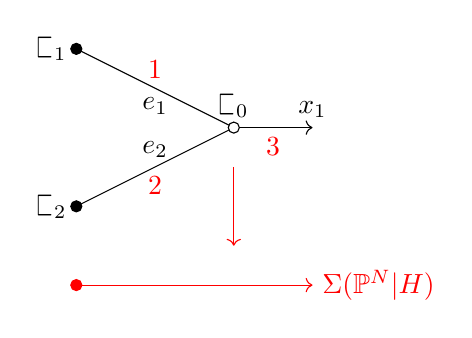
\begin{tikzpicture}
\draw [fill] (0,3) circle[radius=2pt];
\draw (0,3) node[left]{$\sqC_1$};
\draw (0,3) -- (2,2);
\draw (1,2.5) node[above,color=red]{$1$};
\draw (1,2.5) node[below]{$e_1$};

\draw [fill] (0,1) circle[radius=2pt];
\draw (0,1) node[left]{$\sqC_2$};
\draw (0,1) -- (2,2);
\draw (1,1.5) node[below,color=red]{$2$};
\draw (1,1.5) node[above]{$e_2$};

\draw [->] (2,2) -- (3,2);
\draw (3,2) node[above]{$x_1$};
\draw (2.5,2) node[below,red]{$3$};

\draw [fill=white] (2,2) circle[radius=2pt];
\draw (2,2) node[above]{$\sqC_0$};

\draw [->,color=red] (2,1.5) -- (2,0.5);

\draw [->,color=red] (0,0) -- (3,0);
\draw (0,0) [fill=red,color=red] circle[radius=2pt];
\draw (3,0) node[right,color=red]{$\Sigma(\PP^N|H)$};
\end{tikzpicture}
\end{center}
Here each edge (corresponding to a node of the curve) has a length $e_i$ and an expansion factor $u_i$ (indicated in red). The moduli space of such tropical maps is generated by the edge lengths $e_1$ and $e_2$
\begin{equation*} (\RR_{\geq 0})_{e_1} \times (\RR_{\geq 0})_{e_2} \end{equation*}
subject to the continuity condition $e_1=2e_2$. So the tropical moduli space is simply $\RR_{\geq 0}$ generated by $e_2$. Note that for any $e_2 > 0$ (i.e. on the interior of the cone) we have:
\begin{equation*} \lambda(\sqC_2) = e_2 = e_1/2 < e_1 = \lambda(\sqC_1). \end{equation*}
Thus, any logarithmic map with combinatorial type given by the above picture is automatically aligned. This means that the map $\VZ \to \Mcal$ is an isomorphism in a neighbourhood of our chosen element (there is no blowing up necessary). Indeed, the tropical moduli space is $\RR_{\geq 0}$ and this cone does not admit a polyhedral subdivision (there is no non-trivial toric blow-up of $\Aaff^1$).
\end{example}

\begin{example}
Consider now an element of $\Mcal$ whose associated tropical map has the corresponding combinatorial type:
\begin{center}
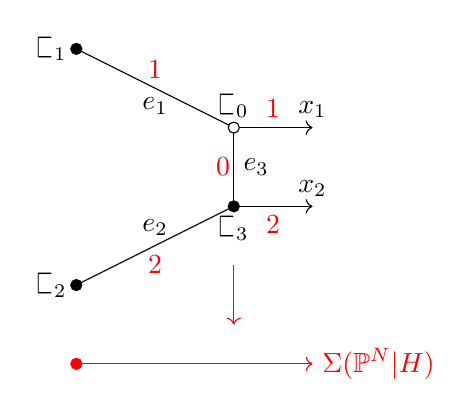
\begin{tikzpicture}
\draw [fill] (0,4) circle[radius=2pt];
\draw (0,4) node[left]{$\sqC_1$};
\draw (0,4) -- (2,3);
\draw (1,3.5) node[above,color=red]{$1$};
\draw (1,3.5) node[below]{$e_1$};

\draw [fill] (0,1) circle[radius=2pt];
\draw (0,1) node[left]{$\sqC_2$};
\draw (0,1) -- (2,2);
\draw (1,1.5) node[below,color=red]{$2$};
\draw (1,1.5) node[above]{$e_2$};

\draw [->] (2,3) -- (3,3);
\draw (3,3) node[above]{$x_1$};
\draw (2.5,3) node[above,red]{$1$};

\draw (2,3) -- (2,2);
\draw [fill] (2,2) circle[radius=2pt];
\draw (2,2.5) node[right]{$e_3$};
\draw (2.075,2.5) node[left,red]{$0$};
\draw (2,2) node[below]{$\sqC_3$};

\draw [->] (2,2) -- (3,2);
\draw (3,2) node[above]{$x_2$};
\draw (2.5,2) node[below,red]{$2$};

\draw [fill=white] (2,3) circle[radius=2pt];
\draw (2,3) node[above]{$\sqC_0$};

\draw [->,color=red] (2,1.25) -- (2,0.5);

\draw [->,color=red] (0,0) -- (3,0);
\draw (0,0) [fill=red,color=red] circle[radius=2pt];
\draw (3,0) node[right,color=red]{$\Sigma(\PP^N|H)$};
\end{tikzpicture}
\end{center}
As before, expansion factors are indicated in red and the edge lengths are $e_1,e_2,e_3$. The tropical moduli space is $\RR_{\geq 0}^3$ generated by these three lengths, subject to the continuity condition $e_1=2e_2$. Thus the moduli space is isomorphic to $\RR_{\geq 0}^2$ generated by $e_2$ and $e_3$. In order to have an alignment, at least one of $\lambda(\sqC_1)$ and $\lambda(\sqC_2)$ must be equal to the radius $\delta$. Note that
\begin{align*} \lambda(\sqC_1) & = e_1 = 2e_2 \\
\lambda(\sqC_2) & = e_2 + e_3\end{align*}
and without more information we cannot say which of these is larger. The subdivision of $(\RR_{\geq 0})^2$ is obtained by dividing the cone into regions where different order relations hold amongst the distances $\lambda(\sqC_1),\lambda(\sqC_2),\lambda(\sqC_3)$. The walls of this subdivison correspond to where some of these distances are equal. Note that in this setting we always have $\lambda(\sqC_2) > \lambda(\sqC_3)$ (at least, as long as we remain in the interior of the cone). The remaining possibilities are:
\begin{align*} \lambda(\sqC_1) & = \lambda(\sqC_3) \qquad (\Leftrightarrow e_1 = e_3 \Leftrightarrow 2e_2 = e_3) \\
\lambda(\sqC_1) & = \lambda(\sqC_2) \qquad (\Leftrightarrow e_1 = e_2 + e_3 \Leftrightarrow e_2 = e_3). \end{align*}
Thus, the subdivision of the tropical moduli space $(\RR_{\geq 0}^2)_{e_2 e_3}$ is given by:
\begin{center}
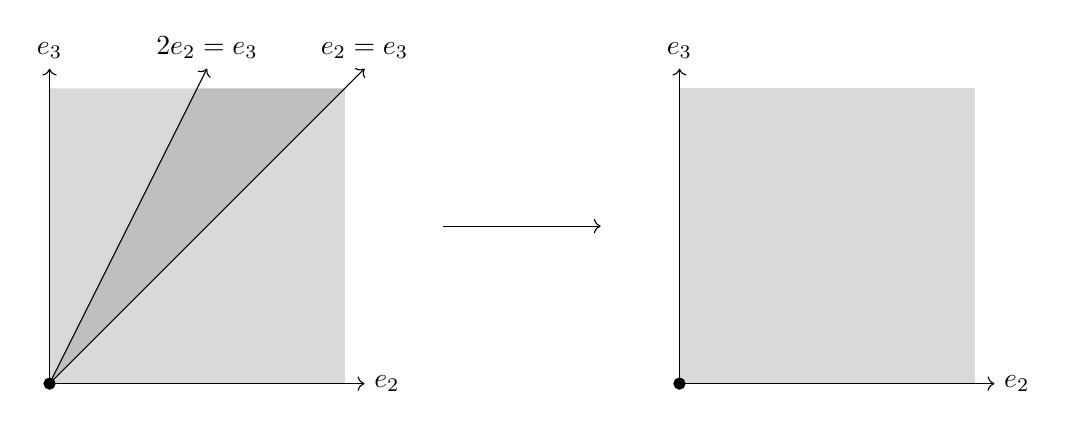
\begin{tikzpicture}[scale=1]
% Right-hand box
\fill [fill=gray!30!white] (5,0) -- (8.75,0) -- (8.75,3.75) -- (5,3.75) -- cycle;
\draw [fill] (5,0) circle[radius=2pt];
\draw [->] (5,0) -- (9,0);
\draw (9,0) node[right]{$e_2$};
\draw [->] (5,0) -- (5,4);
\draw (5,4) node[above]{$e_3$};

% Left-hand box
\fill [fill=gray!30!white] (-3,0) -- (0.75,0) -- (0.75,3.75) -- cycle;
\fill [fill=gray!50!white] (-3,0) -- (0.75,3.75) -- (-1.125,3.75) -- cycle;
\fill [fill=gray!30!white] (-3,0) -- (-1.125,3.75) -- (-3,3.75) -- cycle;
\draw [fill] (-3,0) circle[radius=2pt];
\draw [->] (-3,0) -- (1,0);
\draw (1,0) node[right]{$e_2$};
\draw [->] (-3,0) -- (-3,4);
\draw (-3,4) node[above]{$e_3$};

% 2e_2=e_3 line
\draw [->] (-3,0) -- (-1,4);
\draw (-1,4) node[above]{$2e_2=e_3$};

% e_2=e_3 line
\draw [->] (-3,0) -- (1,4);
\draw (1,4) node[above]{$e_2=e_3$};

% arrow
\draw [->] (2,2) -- (4,2);
\end{tikzpicture}
\end{center}
The cones of the subdivison index the logarithmic strata in a neighbourhood of the preimage in $\VZ$ of our chosen element of $\Mcal$. These can be described as follows:
\begin{center}
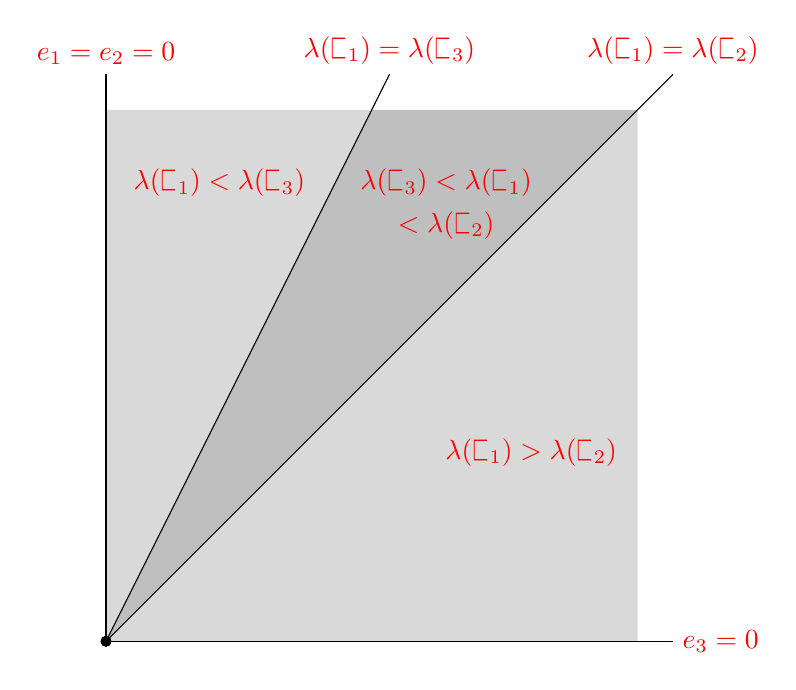
\begin{tikzpicture}[scale=1.8]
% Left-hand box
\fill [fill=gray!30!white] (-3,0) -- (0.75,0) -- (0.75,3.75) -- cycle;
\fill [fill=gray!50!white] (-3,0) -- (0.75,3.75) -- (-1.125,3.75) -- cycle;
\fill [fill=gray!30!white] (-3,0) -- (-1.125,3.75) -- (-3,3.75) -- cycle;
\draw [fill] (-3,0) circle[radius=1pt];
\draw (-3,0) -- (1,0);
\draw (1,0) node[right,red]{$e_3=0$};
\draw (-3,0) -- (-3,4);
\draw (-3,4) node[above,red]{$e_1=e_2=0$};

% 2e_2=e_3 line
\draw (-3,0) -- (-1,4);
\draw (-1,4) node[above,red]{$\lambda(\sqC_1)=\lambda(\sqC_3)$};

% e_2=e_3 line
\draw (-3,0) -- (1,4);
\draw (1,4) node[above,red]{$\lambda(\sqC_1)=\lambda(\sqC_2)$};

\draw (0,1.5) node[below,red]{$\lambda(\sqC_1) > \lambda(\sqC_2)$};

\draw (-0.6,3.4) node[below,red]{$\lambda(\sqC_3) < \lambda(\sqC_1)$};
\draw (-0.6,3.1) node[below,red]{$< \lambda(\sqC_2)$};

\draw (-2.2,3.4) node[below,red]{$\lambda(\sqC_1) < \lambda(\sqC_3)$};
\end{tikzpicture}
\end{center}
There are four codimension--$1$ logarithmic strata of $\VZ$ intersecting our chosen neighbourhood, corresponding to the rays in the above picture. Two of these -- those corresponding to the rays labeled $\{ e_1=e_2=0 \}$ and $\{ e_3=0 \}$ -- are the proper transforms of codimension--$1$ strata in $\Mcal$. These strata consist of log stable maps where some of the tropical edge lengths are equal to zero, meaning that the corresponding nodes have been smoothed. Notice that although the curve has three nodes, there are only two such strata: the nodes $q_1$ and $q_2$ cannot be smoothed independently because of the relation $e_1=2e_2$.

The remaining two codimension--$1$ strata in $\VZ$ -- corresponding to the interior rays in the above picture -- consist of log stable maps where some of the vertex distances become equal. Here none of the nodes are smoothed. From the construction of the subdivision, we see that both these strata map onto a codimension--$2$ stratum of $\Mcal$ (namely, the locus in which all of the nodes persist); this coheres with the fact that they should be thought of as exceptional loci of the blow-up. The extra dimension of moduli comes from the choice of alignment.

Finally, there are three codimension--$2$ strata, corresponding to different \emph{strict} orderings of the vertex distances. Note that the divisorial strata corresponding to $\{e_1=e_2=0\}$ and $\{e_3=0\}$, which intersected in $\Mcal$, no longer intersect in $\VZ$, since we have blown up. The picture is something like:
\begin{center}
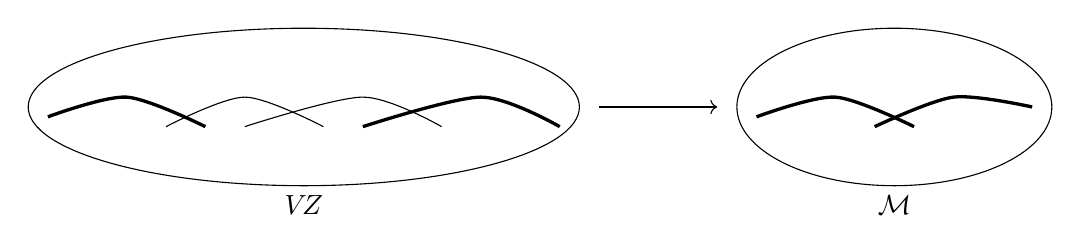
\begin{tikzpicture}[scale=0.5]
\draw (-6.5,0.5) ellipse (4 and 2);
\draw (-6.5,-1.5) node[below]{$\Mcal$};
\draw [very thick] plot [smooth] coordinates{(-10,0.25) (-8,0.75) (-6,0)};
\draw [very thick] plot [smooth] coordinates{(-7,0) (-5,0.75) (-3,0.5)};

\draw (-21.5,0.5) ellipse (7 and 2);
\draw (-21.5,-1.5) node[below]{$\VZ$};
\draw [very thick] plot [smooth] coordinates{(-28,0.25) (-26,0.75) (-24,0)};
\draw plot [smooth] coordinates{(-25,0) (-23,0.75) (-21,0)};
\draw plot [smooth] coordinates{(-23,0) (-20,0.75) (-18,0)};
\draw [very thick] plot [smooth] coordinates{(-20,0) (-17,0.75) (-15,0)};

\draw [->] (-14,0.5) -- (-11,0.5);
\end{tikzpicture}
\end{center}

\end{example}

\subsection{Global logarithmic strata}
In the previous subsections we used tropical geometry to identify the logarithmic strata of $\VZ=\VZ_{1,\alpha}(\PP^N|H,d)$ local to the preimage of a point in $\Mcal$. In fact, the whole discussion carries over if we replace a point in $\Mcal$ by a locally closed logarithmic stratum: the key observation is simply that the tropical moduli space does not vary if we move inside a locally closed logarithmic stratum, so the subdivision process makes sense over that whole stratum. This fact will allow us to describe the logarithmic strata of $\VZ$ globally.

\subsubsection{Logarithmic strata of $\Mcal$} The locally closed logarithmic strata of $\Mcal$ consist of loci where the combinatorial type of the associated tropical curve is constant\footnote{(Navid) Reference for this?}. This is because the combinatorial type determines the minimal monoid $Q$, which coincides with the stalk of the ghost sheaf on $\Mcal$.

If we have two strata $\Scal_1$ and $\Scal_2$ corresponding to combinatorial types $\Delta_1$ and $\Delta_2$, then $\Scal_2$ is contained in the closure of $\Scal_1$ if and only if the combinatorial type $\Delta_1$ is obtained from $\Delta_2$ by a process of generisation: namely, by contracting some edges (i.e. smoothing some nodes) and moving some of the vertices from the interior $\RR_{>0} \subseteq \RR_{\geq 0}$ of the tropicalisation $\Sigma(\PP^N|H)$ to the vertex $0 \in \RR_{\geq 0}$ (i.e. moving some components of the curve outside $H$). This allows us to completely describe the dual intersection complex of the logarithmic strata of $\Mcal$.

Note that we are \emph{not} able to easily read off the codimension of a logarithmic stratum from the combinatorial data: the codimension of the associated stratum in the Artin fan $\Acal_\Mcal$ is given by the dimension of the tropical moduli space, but the map $\Mcal\to\Acal_\Mcal$ is not smooth (since $\Mcal$ is not log smooth) so we are not able to say anything about the locus in $\Mcal$. 

\subsubsection{Logarithmic strata of $\VZ$}
Now let us pick a stratum $\Scal \subseteq \Mcal$ indexed by a combinatorial type $\Delta$ and with associated monoid $Q$. We may choose a sufficiently small open neighbourhood of $\Scal$ which only intersects logarithmic strata $\Scal^\prime$ which contain $\Scal$ in their closures. The previous discussion then shows that if we pick any point in this open neighbourhood, the combinatorial type of the associated tropical curve is obtained from $\Delta$ by contracting some edges and specialising some vertices. Thus we see that the associated map on tropical moduli spaces is injective, and so the generisation map on the level of ghost sheaves is surjective. This allows us to produce a chart on the open neighbourhood of $\Scal$ with monoid given by $Q$.

The discussion in the previous subsections then applies \emph{mutatis mutandis} to this open set, giving a description of the logarithmic strata of $\VZ$ which intersect an open neighbourhood of the preimage of $\Scal$. Since log strata must map to log strata, this gives a procedure for enumerating all of the locally closed logarithmic strata of $\VZ$, namely:\medskip
\begin{enumerate}
\item Enumerate the locally closed logarithmic strata of $\Mcal$ by enumerating all possible combinatorial types of tropical curves with the given numerical data. The dual intersection complex of these strata is specified by generisation of combinatorial types, as described earlier.\medskip
\item For each locally closed stratum $\Scal\subseteq \Mcal$ identify the tropical moduli space $Q^\vee_{\RR}$ associated to the given combinatorial type, and perform the subdivision specified by the alignment condition. The arguments of the previous subsections carry over to give a description of the logarithmic strata of $\VZ$ which map to a neighbourhood of $\Scal$. The dual intersection complex of these strata is specified by the combinatorics of each subdivision together with the dual intersection complex of the strata of $\Mcal$.
\end{enumerate}
We now illustrate this is in some examples:
\begin{example} Example of low-degree computation of logarithmic strata. (Note that for $\Mcal$ we can't read off the codimension from the dimension of the tropical moduli space because $\Mcal$ is not log smooth.)\footnote{(Navid) To be done.}\end{example}


\newpage

\section{Splitting axiom and recursion formula for $(\PP^N|H)$}

\noindent  In the previous section we explained how to determine the logarithmic strata of $\VZ$. We now focus our attention on certain logarithmic divisors, providing a recursive description for these loci: that is, a description in terms of fibre products of smaller moduli spaces. This is the technically most difficult part of the paper. The recursive description bears some similarities with the recursive description of the boundary of the absolute space $\VZ_{1,n}(\PP^N,d)$ given in \cite{VZ}; in keeping with the theme of this paper, however, we will see that log geometry provides a convenient framework for dealing with the combinatorics.

The end result is that we obtain an explicit formula for tautological integrals over these boundary loci. This produces a Gathmann recursion  for relative invariants in genus one.

The plan for this section is as follows \footnote{(Navid) Finish this}

\subsection{Recursion setup} Consider an element of $\VZ$ and choose a marked point $x_k\in C$. We note that by the existence of a log morphism, either $f$ has contact order $\alpha_k$ to $H$ at the marking $x_k$, or else the irreducible component of $C$ containing $x_k$ is mapped entirely inside $H$ (we say ``$x_k$ belongs to an internal component'' in this case).

By pulling back the equation defining $H$ along $f$ and then taking its $\alpha_k$-th derivative at $x_k$ (which makes sense since all the lower-order derivatives vanish by assumption) we obtain a section of a jet bundle on $\VZ$ whose vanishing locus coincides (set-theoretically) with the locus where $x_k$ belongs to an internal component. As in \cite[Construction 2.1]{Ga} there is an exact sequence of jet bundles
\begin{equation*} 0\to x_k^\st\omega_{\mathcal{C}/\VZ}^{\otimes\alpha_k}\otimes\ev_k^\st\OO_{\PP^N}(H)\to x_k^\st\mathcal J^{\alpha_k}(f^\st\OO_{\PP^N}(H))\to x_k^\st\mathcal J^{\alpha_k-1}(f^\st\OO_{\PP^N}(H))\to 0 \end{equation*}
and thus we obtain a section of the line bundle $x_k^\st\omega_{\mathcal{C}/\VZ}^{\otimes\alpha_k}\otimes\ev_k^\st\OO_{\PP^N}(H)$ with vanishing locus equal to the locus where $x_k$ belongs to an internal component. Writing this locus as
\begin{equation*} \Dcal(k) = \Dcal_{1,\alpha}^k(\PP^N|H,d) \subseteq \VZ_{1,\alpha}(\PP^N|H,d) = \VZ \end{equation*}
we obtain:
\begin{lem} $(\alpha_k\psi_k+\ev_k^\st H)\cap[\VZ]=[\Dcal(k)].\footnote{(Navid) Should we work out the vanishing orders of the section at this point?}$\end{lem}
\noindent The remainder of this section will be devoted to providing an explicit recursive description of the class $[\Dcal(k)]$ in terms of tautological classes on spaces of maps with smaller numerical invariants. As we will see, this provides an algorithm for computing reduced relative invariants, as well as a quantum Lefschetz algorithm for reduced (absolute) invariants in genus one.

\subsection{Identifying the irreducible components of $\Dcal(k)$} Here we explain the strategy for identifying the irreducible components of $\Dcal(k)$ via tropical geometry.

\begin{lemma} Every irreducible component of $\Dcal(k)$ is a codimension-$1$ logarithmic stratum.\end{lemma}
\begin{proof} This is not hard to see: the locus where the log structure is trivial coincides precisely with the  locus where the source curve is smooth and not mapped inside $H$, and since $\VZ$ is log smooth this locus is open and dense. By definition $\Dcal(k)$ is disjoint from this locus, hence is contained in the  complement of this locus, which (by the very definition of logarithmic strata) can be written as a union of logarithmic strata of positive codimension. Since $\Dcal(k)$ has codmension $1$, it must therefore be equal to a union of logarithmic divisors.\end{proof}

In the previous section we discussed at length a procedure for describing the logarithmic strata of $\VZ$. This shows that every divisorial logarithmic stratum is obtained via a three-step process:
\begin{enumerate}
\item choose the combinatorial type of a tropical map;
\item subdivide the corresponding tropical moduli space;
\item choose a ray in this subdivision.
\end{enumerate}
Notice that this process contains some redundancies: once we choose a ray of the tropical moduli space, we obtain a generisation of the intial combinatorial type, given by contracting some edges of the dual graph.

\begin{example} \end{example}

Whenever we consider a logarithmic stratum in $\VZ$, by its combinatorial type we will always mean the generisation of the ``initial'' combinatorial type induced by our choice of cone in the polyhedral subdivision. This does not depend on the choice of initial combinatorial type.

Now, the logarithmic divisors which are contained in $\Dcal(k)$ are precisely those whose corresponding combinatorial type has the vertex of the dual graph containing $x_k$ mapped into the interior $\RR_{>0} \subseteq \RR_{\geq 0}$.

Thus, via the above procedure, we are able to enumerate the irreducible components of $\Dcal(k)$ in a combinatorial manner. The combinatorial type and choice of ray allows us to describe the general element of such a component. What we are still lacking is a recursive description of the components, which we need in order to compute integrals over them. This is the subject of the remainder of this section.

\subsection{Splitting and gluing punctured logarithmic maps}\label{subsection punctured maps} We still start by considering the usual moduli space $\Mcal$ of log stable maps. In \cite{PuncturedMaps}, a recursive description of the logarithmic strata of $\Mcal$ is given, in terms of moduli spaces of punctured maps. As discussed above, the logarithmic strata $\Scal$ of $\Mcal$ are indexed by combinatorial types of tropical curves. Given such a combinatorial type $\Delta$, each vertex $v$ of the associated graph defines a moduli space of punctured stable maps:
\begin{equation*} \ol\Mcal_v = \Mpunct{g(v)}{\alpha(v)}{Z_v}{d(v)}. \end{equation*}
Here $g(v)$ and $d(v)$ are the genus and degree assigned to the vertex, while $Z_v$ is the logarithmic stratum of the target corresponding to the tropical stratum into which the vertex is mapped by the combinatorial type (in our setting, $Z_v=\PP^N$ or $H$). The length of the vector $\alpha(v)$ is given by the number of flags adjacent to $v$, and the entries (which represent tangencies, and may be positive or negative) are given by the expansion factors along those flags. If all of the tangencies are positive, then this is nothing but an ordinary moduli space of log stable maps.

The corresponding logarithmic stratum is then obtained as a follows. For each vertex $v$ and each adjacent flag $E \ni v$ we define $\widetilde\Mcal_v^E$ to be the stack $\ol\Mcal_v$ equipped with the log structure
\begin{equation*} p_{v,E}^\st \Mcal_{\Ccal_v^\circ} \end{equation*}
where $p_{v,E} \colon \ol\Mcal_v \to \Ccal_v^\circ$ is the marking section corresponding to $E$. This definition makes $p_{v,E}$ into a strict logarithmic map, and composing with the universal map produces a logarithmic evaluation morphism $\ev_{v,E} \colon \widetilde\Mcal_v^E \to Z_E$, where $Z_E \subseteq Z_v$ is the logarithmic stratum into which the marking corresponding to $E$ is mapped.

If $E_1,\ldots,E_k$ are the flags adjacent to $v$ then we define
\begin{equation*} \widetilde\Mcal_v = \widetilde\Mcal_v^{E_1} \times_{\ol\Mcal_v} \ldots \times_{\ol\Mcal_v} \widetilde\Mcal_v^{E_k} \end{equation*}
where the fibre product is taken in the fs log category. With this definition, all the evaluation maps $\ev_{v,E} \colon \widetilde{\Mcal}_v \to Z_E$ are naturally logarithmic morphisms. Then the corresponding logarithmic stratum is obtained by taking the following fibre product (again, in the fs log category):
\bcd
\Scal \ar[r] \ar[d] \ar[rd,phantom,"\square"] & \prod_v \widetilde\Mcal_v \ar[d] \\
\prod_{E} Z_E \ar[r] & \prod_{E} Z_E \times Z_E.
\ecd
In the above discussion, there were two steps at which we needed to take fs fibre products: first, when constructing each $\widetilde{\Mcal}_v$ and second, when construction $\Scal$. Typically the fs fibre product does not agree with the usual fibre product of stacks; rather, one must take the fibre product in the category of coherent log stacks (which \emph{does} agree with the usual fibre product) and then integralise and saturate the result.

We will now argue that in our situation, when we take fibre products of coherent log stacks, the result is automatically integral. This means that the integralisation process is redundant, and so the fs fibre product is obtained from the ordinary fibre product by a process of saturation. This amounts to taking a finite cover of the underlying stack (whose degree we will compute).

The following lemma holds for arbitrary moduli spaces of punctured maps.

\begin{lemma} Given a combinatorial type $\Delta$ indexing a stratum of $\Mcal$ and a vertex $v$ of the associated graph, consider the corresponding moduli space of punctured stable maps $\ol\Mcal_v$. As in the above discussion, define for each adjacent flag $E \ni v$ the log stack $\widetilde\Mcal_v^E$ by pulling back the log structure of the punctured curve along the marking section. Consider the fibre product \emph{in the category of coherent log stacks}:
\begin{equation*} \widetilde\Mcal^{\operatorname{not-fs}}_v = \widetilde{\Mcal}_v^{E_1} \times_{\ol\Mcal_v} \ldots \times_{\ol\Mcal_v} \widetilde{\Mcal}_v^{E_k}. \end{equation*}
Then $\widetilde\Mcal^{\operatorname{not-fs}}_v$ is integral (and consequently, the map $\widetilde\Mcal_v \to \widetilde\Mcal^{\operatorname{not-fs}}_v$ is finite).
\end{lemma}
\begin{proof} Locally we have a chart for $\ol\Mcal_v$ given by $Q$ (the minimal monoid as constructed, for instance, in \cite[Construction 1.16]{GrossSiebertLog}) and charts for $\widetilde\Mcal_v^{E_i}$ given by $Q_{E_i}$, where $Q_{E_i} = Q \oplus \N$ if $E_i$ corresponds to an ordinary marked point, and $Q_{E_i}$ is the submonoid of $Q \oplus \Z$ generated by $Q \oplus \N$ and $(\ol\varphi_{\eta_i}(1),u_{E_i})$ if $E_i$ corresponds to a puncturing (so that $u_{E_i} \in \Z_{<0}$). In either case, we have $Q_{E_i} \subseteq Q \oplus \Z \subseteq Q^{\operatorname{gp}} \oplus \Z$ (since $Q$ is integral) and so $Q_{E_i}$ is integral (recall that a monoid is integral if and only if it admits an injective homomorphism into a group). In this notation, $\widetilde\Mcal_v^{\operatorname{not-fs}}$ admits a chart given by the monoid:
\begin{equation*} P = Q_{E_1} \oplus_Q Q_{E_2} \oplus_Q \ldots \oplus_Q Q_{E_k}.\end{equation*}
Suppose without loss of generality that $E_1,\ldots,E_r$ are punctures and $E_{r+1},\ldots,E_k$ are ordinary marked points; then $P$ is equal to the submonoid of
\begin{equation*} Q \times \Z^r \times \N^{k-r} \end{equation*}
generated by $Q \times \N^k$ and $(\ol\varphi_{\eta_i}(1),u_{E_i} e_i,0)$ for $i\in \{1,\ldots,r\}$, where $e_i \in \Z^r$ is the $i$th basis element and $0 \in \N^r$. In particular, $P$ admits an injective homomorphism into the group
\begin{equation*} Q^{\gp} \times \Z^r \times \Z^{k-r} \end{equation*}
and hence is integral.\end{proof}

\footnote{(Navid) Is this a good point to calculate the degree of $\widetilde\Mcal_v \to \widetilde\Mcal_v^{\operatorname{not-fs}}$?}The previous lemma holds for arbitrary moduli spaces of punctured maps. The next lemma, on the other hand, is special to our setting.

\begin{lemma} Consider the fibre product in the category of coherent log stacks:
\bcd
\Scal^{\operatorname{not-fs}} \ar[r] \ar[d] \ar[rd,phantom,"\square"] & \prod_v \widetilde\Mcal_v \ar[d] \\
\prod_{E} Z_E \ar[r] & \prod_{E} Z_E \times Z_E.
\ecd
Then $\Scal^{\operatorname{not-fs}}$ is integral.\end{lemma}
\begin{proof}\end{proof}


This gives a recursion description of the logarithmic strata in $\Mcal$. We will now\footnote{(Navid) Really, after the next section, which maybe we should move to an appendix} use this to obtain a similar (though somewhat more complicated) description of the strata in $\VZ$.

\subsection{Punctured maps and double ramification loci}\footnote{(Navid) Move this to an appendix?} We will now present some arguments and constructions aimed at demystifying the moduli spaces of punctured stable maps. In our context, we only ever encounter these spaces when the associated logarithmic stratum $Z_v$ of the target is the divisor $H$. Consider therefore a moduli space of punctured stable maps
\begin{equation}\label{punctured space} \Mpunct{g}{\alpha}{H}{d} \end{equation}
where $g \in \{0,1\}$ and $\alpha$ is a vector of tangency orders. The target $H$ is given the log structure pulled back from $\PP^N$, and consequently is not log smooth. As such, the natural obstruction theory on the above moduli space will not, in general, be perfect. This is not really a problem for us, since we are mainly interested in studying the non-virtual geometry of our moduli spaces. Indeed, we will see that the space \eqref{punctured space} is birational to the moduli space of ordinary stable maps to $H$ satisfying the condition:
\begin{equation}\label{DRC condition} f^\st[H] - \sum_{i=1}^n \alpha_ix_i =0 \in \Achow_0(C).\end{equation}
This space forms a closed substack
\begin{equation*} \ol\Mcal^{\alpha}_{g,n}(H,d) \subseteq \M{g}{n}{H}{d} \end{equation*}
and is referred to as the \emph{double ramification locus}. These moduli spaces have been the focus of intense study over the years (see, for instance, \cite{GathmannThesis} \cite{DRCBundle}). The double ramification locus is a closed substack of $\M{g}{n}{H}{d}$ of virtual codimension $g$ (though, as with $\M{g}{n}{H}{d}$ itself, it typically has excess dimension).

\begin{prop} Suppose that $g \in \{0,1\}$ and consider the morphism forgetting all log structures:
\begin{equation*} \Mpunct{g}{\alpha}{H}{d} \to \M{g}{n}{H}{d}. \end{equation*}
This factors through the double ramification locus, and is in fact birational onto its image.\end{prop}
\begin{proof} The fact that the forgetful morphism factors through the double ramification locus is an immediate consequence of the balancing condition satisfied by punctured stable maps, interpreted as a condition in $\Pic(C)$ (the more familiar balancing condition is obtained from this one by restricting to a component of $C$ and then taking degrees). Thus indeed we have a map:
\begin{equation*} \varphi \colon \Mpunct{g}{\alpha}{H}{d} \to \ol\Mcal^\alpha_{g,n}(H,d). \end{equation*}
To show that $\varphi$ is birational, we will choose an open dense locus of the domain and show that $\varphi$ induces an isomorphism on geometric points when restricted to this locus. The locus we take is the preimage of the locus inside $\ol\Mcal^\alpha_{g,n}(H,d)$ consisting of curves of compact type (i.e. those whose dual graph has genus zero); essentially we are excluding stable maps whose source curve contains a cycle of $\PP^1$s. The fact that this is open dense in $\ol\Mcal^\alpha_{g,n}(H,d)$ is not hard to see: when $g=1$ (the only case in which non-compact type curves can arise), the double ramification locus contains many components, but on every such component the maximal genus one subcurve of the source will be generically smooth, which shows again that the locus of stable maps not of compact type is closed inside $\ol\Mcal^\alpha_{g,n}(H,d)$. Once we show that $\varphi$ is bijective on geometric points when restricted to the preimage of this locus, it follows (since $\varphi$ is a finite morphism) that the preimage of this locus is dense in $\Mpunct{g}{\alpha}{H}{d}$, and hence that $\varphi$ is birational.

So, let us start with a compact type stable map which belongs to the double ramification locus:
\bcd
C \ar[r,"f"] \ar[d] & H \\
S=\Spec\kfield
\ecd
We will show that there exists a unique lift of this to a punctured stable map. Since $C$ has compact type, there is a unique choice of associated combinatorial type $\Delta$. This determines a minimal monoid $Q$ such that any punctured map enhancing the given stable map has base log structure given by:
\begin{align*}
Q \oplus \kfield^\st & \to \kfield \\
(q,\lambda) & \mapsto \begin{cases} \lambda \qquad \text{if } q =0 \\ 0 \qquad \text{otherwise} \end{cases}
\end{align*}
If we let $r$ denote the number of nodes of $C$ then by construction there is a natural map $\N^r \to Q$ and by the universal property of minimality our punctured curve must be obtained by puncturing a log smooth curve pulled back along a morphism of log schemes:
\begin{equation*} (\Spec\kfield,Q \oplus \kfield^\st) \to (\Spec\kfield,\N^r\oplus\kfield^\st).\end{equation*}
This log morphism must enhance the given map $\N^r \to Q$ on the level of ghost sheaves. The moduli for such a log map is $\Gm^r$, but all these choices are canceled out by automorphisms of $(\Spec\kfield,Q\oplus\kfield^\st)$\footnote{(Navid) Here we are using the fact that $Q$ is in some sense bigger than $\N^r$.}. Thus we obtain, by pulling back the minimal log smooth curve over $(\Spec\kfield,\N^r \oplus\kfield^\st)$, a unique log smooth curve:
\begin{equation*} (C,\Mcal_C) \to (\Spec\kfield,Q\oplus\kfield^\st).\end{equation*}
We must now construct the puncturing $\Mcal_{C^\circ}$. Let $\Pcal_C$ denote the divisorial log structure on $C$ with respect to the punctures. It is easy to see that there is a unique log structure $\Mcal$ on $C$ such that
\begin{equation*} \Mcal_C = \Mcal \oplus_{\OO_C^\st} \Pcal_C \end{equation*}
where the pushout is taken in the category of monoid sheaves. We consider the sheaf:
\begin{equation*} \Ncal_C = \Mcal \oplus_{\OO_C^\st} \Pcal^{\gp}_C. \end{equation*}
By definition the puncturing $\Mcal_{C^\circ}$ should be an intermediate sheaf:
\begin{equation*} \Mcal_C \subseteq \Mcal_{C^\circ} \subseteq \Ncal_C. \end{equation*}
We will now construct this, and argue that our construction gives the only puncturing possible. First we note that it is sufficient to define $\Mcal_{C^\circ}$ on a base for the topology on $C$. We choose a base such that for each base open set $U$:
\begin{enumerate}
\item $U$ is connected;
\item $U$ contains at most one of the punctures of $C$;
\item if $U$ contains a puncture $p \in C$, then $U$ does not contain any of the nodes or markings of $C$, and $\OO_C(p)|_U$ is trivial.
\end{enumerate}
Note that these properties are stable under taking subsets, so to obtain such a base we simply choose an open cover with this property (which is certainly possible) and then take the collection of all open subsets of our chosen cover.

Now let $U$ be such an open set in our base. If $U$ does not contain a puncture then $\Mcal_C|_U = \Ncal_C|_U$ and so we set
\begin{equation*} \Mcal_{C^\circ}(U) = \Mcal_C(U).\end{equation*}
If $U$ contains a puncture $p$ then by assumption $U \setminus \{ p\}$ contains only smooth unmarked points, and hence we have a splitting
\begin{equation*} \Ncal_C|_U = \left( \pi^\st \Mcal_S|_U \right) \oplus_{\OO_U^\st} \left(\Pcal_p^{\gp}|_U \right) \end{equation*}
where $\Pcal_p$ is the divisorial log structure with respect to $p$. Since $\Mcal_S = Q \oplus \kfield^\st$ it follows that $\pi^\st\Mcal_S|_U = \ul{Q} \oplus \OO_U^\st$. Thus we see that
\begin{equation*} \Ncal_C|_U = \ul{Q} \oplus \Pcal_p^{\gp}|_U\end{equation*}
and similarly:
\begin{equation*} \Mcal_C|_U = \ul{Q} \oplus \Pcal_p|_U.\end{equation*}
We therefore have (since $U$ is connected):
\begin{equation*} \Ncal_C(U) = Q \oplus \Pcal_p^{\gp}(U) \end{equation*}
Recall we are assuming that $\OO_C(p)|_U$ is trivial. Choosing a trivialisation, we obtain a function $s \in \OO_U(U)$ such that $p=\{s=0\}$ on $U$. Then $\Pcal_p(U)$ consists of functions of the form $\lambda \cdot s^n$ for $n \in \N$ and $\lambda \in \OO_U^\st(U)$. Groupifying, we obtain:
\begin{equation*} \Pcal^{\gp}_p(U) = \left\{ \lambda \cdot s^k \, \vert \, \lambda \in \OO_U^\st(U), k \in \Z \right\}. \end{equation*}
(Indeed, $\Pcal_p^{\gp}$ can be described as the sheaf of rational functions which are regular and invertible outside of $p$.) Recall that $p$ has attached to it a tangency order $\alpha_p \in \Z_{<0}$. If we let $\eta$ denote the generic point of the component of $C$ containing $p$, then we also have a pullback map $\ol\varphi_\eta \colon \N \to Q$ which is sharp (i.e. it is not the zero map). We define $\Mcal_{C^\circ}(U) \subseteq \Ncal_C(U)$ to be the submonoid generated by $Q \oplus \Pcal_p(U)$ and the element:
\begin{equation*} (\ol\varphi_\eta(1),s^{\alpha_p}). \end{equation*}
This clearly satisfies the conditions to be a puncturing, and by the prestability condition it is the only possibility for $\Mcal_{C^\circ}$. We thus have a punctured curve:
\begin{equation*} (C,\Mcal_{C^\circ}) \to (C,\Mcal_C) \to (\Spec\kfield,Q\oplus\kfield^\st). \end{equation*}
It remains to construct the log enhancement of the map $f \colon C \to H$. The map $f^\flat \colon f^\st \Mcal_H \to \Mcal_{C^\circ}$ is already determined on the level of ghost sheaves. To enhance this to a map on the level of log structures entails choosing an isomorphism of line bundles:
\begin{equation*} f^\st \OO_H(1) \cong \OO_C\left(\ol{f}^\flat(1)\right). \end{equation*}
The component-wise description of the right-hand side in \cite{RSPW} (together with the fact that $C$ is compact type, so its Picard group is simply the product of the Picard groups of its components) shows that such an isomorphism exists if and only if the original stable map is in the double ramification locus. There is a $\Gm$ worth of choices for such a map, but these are canceled out by the automorphisms of $(C,\Mcal_{C^\circ})$ induced by pulling back along (strict) automorphisms of $(\Spec\kfield,Q\oplus\kfield^\st)$. This completes the proof of unique punctured lifting.
\end{proof}

Thus, the spaces of punctured maps we encounter are always birational to double ramification loci. We now briefly discuss the geometry of these loci. In the genus zero case, the double ramification locus is equal to the entire space
\begin{equation*} \ol\Mcal^{\alpha}_{0,n}(H,d) = \M{0}{n}{H}{d} \end{equation*}
which is smooth. Thus tautological integrals over $\ol\Mcal^{\alpha}_{0,n}(H,d)$ are determined by the genus-zero Gromov--Witten theory of $H$.

The genus one case is more delicate: there is a ``main component'' of the double ramification locus, obtained as the closure of the locus where the source curve is smooth. This forms a divisor inside the main component of the moduli space of stable maps:
\begin{equation*} \ol\Mcal^{\alpha,\circ}_{1,n}(H,d) \subseteq \ol\Mcal^\circ_{1,n}(H,d). \end{equation*}
However, we know that $\M{1}{n}{H}{d}$ contains many other components besides $\ol\Mcal^\circ_{1,n}(H,d)$, some of which have excess dimension. Certainly the double ramification locus intersects these other components, and sometimes it can do so in quite dramatic fashion. For instance, consider the locus where the source curve splits into a contracted elliptic component and a rational component containing all the markings. This locus forms an irreducible component of the moduli space, isomorphic to
\begin{equation*}\ol\Mcal_{1,1} \times \M{0}{n+1}{H}{d} \end{equation*}
which has excess dimension $N-2$. This entire component belongs to the double ramification locus, since the condition \eqref{DRC condition} becomes entirely numerical here. Thus, we see that the double ramification locus can be quite badly-behaved in genus one. Fortunately, we will only be interested in the main component of this locus (which is birational to the main component of the moduli space of punctured maps); see \S \ref{} below.

\subsection{Recursive description of the divisors: types $A,B$ and $C^+$}

The basic idea is as follows. Choose an irreducible component $\Dcal \subseteq \Dcal(k)$. As discussed above, we can obtain this by choosing an ``initial'' combinatorial type together with a ray of the resulting subdivision of the tropical moduli space. Without loss of generality we may assume that this ``initial'' combinatorial type coincides with the ``true'' combinatorial type of $\Dcal$ obtained by performing the edge contractions specified by the choice of ray.

Since $\VZ \to \Mcal$ is a log modification, the divisor $\Dcal$ is either exceptional or the proper transform of a logarithmic divisor on $\Mcal$. In this subsection, we will focus on the latter case. Then if we let $\Dcal_{\Mcal}^\circ\subseteq \Mcal$ denote the locally closed stratum corresponding to our choice of combinatorial type, and $\Dcal_\Mcal = \overline{\Dcal^\circ_\Mcal}$ denote the corresponding logarithmic divisor in $\Mcal$, then our divisor $\Dcal\subseteq\VZ$ is the proper transform of $\Dcal_\Mcal$, which is obtained by taking the preimage $\Dcal^\circ$ of $\Dcal_\Mcal^\circ$ (since $\Dcal^\circ_\Mcal$ is disjoint from the blown-up locus) and then taking its closure in $\VZ$. This is, of course, different from taking the preimage of $\Dcal_\Mcal$, since in general $\Dcal_\Mcal$ will intersect the blown-up locus. By continuity we have an induced map:
\begin{equation*} \Dcal \to \Dcal_\Mcal. \end{equation*}
The remainder of this section will be dedicated to showing how the map $\Dcal \to \Dcal_\Mcal$ may be interpreted as a blow-up. The reason this is useful is that $\Dcal_\Mcal$ itself has a recursive description in terms of moduli spaces of punctured maps (see \S \ref{subsection punctured maps}), which in our setting we are able to compute integrals over.

For the remainder of this subsection, we will consider only the situation where the circuit is assigned a positive degree by the combinatorial type; the other, more complicated case, will be taken up in \S \ref{}.


\begin{lemma} Let $\Dcal \subseteq \Dcal(k)$ be an irreducible component and let $\Delta$ be the corresponding combinatorial type. Suppose that $\Delta$ assigns positive degree to the circuit. Then $\Delta$ takes one of the following forms:
\begin{figure}[h]
    \centering
    \begin{minipage}{0.3\textwidth}
        \centering
        \Yagraph
        \caption{$\mathcal Y_A$}
    \end{minipage}\hfill
    \begin{minipage}{0.3\textwidth}
        \centering
        \Ybgraph
        \caption{$\mathcal Y_B$}
    \end{minipage}\hfill
    \begin{minipage}{0.3\textwidth}
        \centering
        \Ycgraph
        \caption{$\Ycal_C^+$}
    \end{minipage}
\end{figure}

\noindent The terminology is due to Vakil, and the picture in this case is very similar to \cite{Vre} (as we will see later, when the circuit is contracted the picture becomes \emph{very} different). Note that in these pictures we have omitted the marked points (apart from $x_k$), the degree of each vertex, and the expansion factors of the edges. These combinatorial data can be distributed arbitrarily, as long as:
\begin{enumerate}
\item the vertices $\sqC_1,\ldots,\sqC_r$ have positive degree (and $\sqC_0$ has positive degree in the $\Ycal_C^+$ case);
\item every vertex is stable;
\item the balancing condition is satisfied.
\end{enumerate}\end{lemma}

\begin{proof}
Recall that we have $\Dcal\subseteq\VZ$ obtained by a choice of combinatorial type and ray in the subdivison of the tropical moduli space. In this situation, since the circuit has positive degree no alignment is necessary (both radii are zero), and hence the subdivision is trivial. Following our procedure, we choose a ray of the tropical moduli space $Q^\vee_{\RR}$. Since this is generated by edge lengths, and we are assuming that the initial and generised combinatorial types coincide, we conclude that the tropical moduli space must be $\RR_{\geq 0}$. Since we are assuming that $\Dcal \subseteq \Dcal(k)$, we know that the vertex of the tropicalisation which contains the flag $x_k$ must map into the interior $\RR_{>0}\subseteq \RR_{\geq 0}$.

We claim that this is the only vertex of the tropical curve mapped into the interior; if there were more, the positions of their images in $\RR_{> 0}$ would be independent, and thus the tropical moduli space would have dimension $\geq 2$, a contradiction.\footnote{(Luca) Say something about rigid tropical curves as in ACGS and KLR}

Thus there is a single vertex $\sqC_0$ mapped into the interior $\RR_{>0} \subseteq \RR_{\geq 0}$ and a number of vertices $\sqC_1,\ldots,\sqC_r$ mapped onto the vertex $0 \in \RR_{\geq 0}$. No pair of $\sqC_1,\ldots,\sqC_r$ can be connected by an edge, since this would introduce an extra edge length to the tropical moduli space, which then once again would have dimension $\geq 2$. Each of $\sqC_1,\ldots,\sqC_r$ must have positive degree by the tropical balancing condition and must be connected to $\sqC_0$ (since the tropical curve must be connected).

Thus, we see that the combinatorial type takes the form of a bipartite graph, with $\sqC_0$ on the right-hand side and $\sqC_1,\ldots,\sqC_r$ on the left-hand side. Note that the continuity of the tropical map identifies all of the edge lengths, up to weights given by the expansion factors (i.e. tangency orders) at the edges; thus the tropical moduli space is isomorphic to $\RR_{\geq 0}$ and so we have a divisor as expected.

We distinguish three cases, depending on the position of the circuit, giving the three forms presented in the statement of the lemma.\end{proof}

We now now investigate the three types $A,B,C^+$ separately, giving a recursive description of the boundary locus in each case.


\subsubsection{Type $A$} Let $\Delta$ be a combinatorial type of type $A$ and let $\Dcal\subseteq\VZ$ be the corresponding logarithmic divisor (note there is no choice of ray here). The corresponding locus $\Dcal_\Mcal\subseteq\Mcal$ is given (up to a finite cover) by\footnote{(Navid) Include short appendix on integralisation/saturation when gluing punctured maps in our setting?}:
\begin{equation*}\Dcal_\Mcal=\Mpunct{0}{\alpha^{(0)}\cup (-m_1,\ldots,-m_r)}{H}{d_0}\times_{H^r}\left( \Mlog{1}{\alpha^{(1)}\cup(m_1)}{\PP^N|H}{d_1} \times \prod_{i=2}^r\Mlog{0}{\alpha^{(i)}\cup(m_i)}{\PP^N|H}{d_i} \right). \end{equation*}
\begin{lemma}We have the following description of $\Dcal$\begin{equation}\label{type A splitting axiom}\Dcal=\Mpunct{0}{\alpha^{(0)}\cup (-m_1,\ldots,-m_r)}{H}{d_0}\times_{H^r}\left(\VZ_{1,\alpha^{(1)}\cup(m_1)}(\PP^N|H,d_1)\times\prod_{i=2}^r\Mlog{0}{\alpha^{(i)}\cup(m_i)}{\PP^N|H}{d_i}\right) \end{equation}
i.e. the map $\Dcal\to\Dcal_\Mcal$ is given by blowing up one of the factors of the fibre product.\end{lemma} Note that there is a birational map which forgets the log structures
\begin{equation*} \Mpunct{0}{\alpha^{(0)}\cup(-m_1,\ldots,-m_r)}{H}{d_0} \to \M{0}{n_0+r}{H}{d_0} \end{equation*}
and all of our insertions are pulled back from the latter space. Therefore the integrals over the punctured space are determined by the genus zero Gromov--Witten theory of $H\cong\PP^{N-1}$.

%DEPRECATED?/WRONG?

%Note that if $\sqC_0$ degenerates further then it may be the case that there are components of $\sqC_0$ contained inside the contraction radius for $\sqC$, and thus once we contract to a Smyth curve there are components of $\sqC_0$ adjacent to the genus one singularity. However, in this case when we split off $\sqC_1$ these components disappear, and if the factorisation condition holds for $\sqC$ then it holds a fortiori for $\sqC_1$.\footnote{(Navid) I think this is right, but could someone check? Maybe there's a better way to say this.} Thus we obtain a morphism from $\Dcal$ to the fibre product on the right-hand side of \eqref{type A splitting axiom}.
\begin{proof}
Note first of all that the map $\Dcal\to\Dcal_\Mcal$ is an isomorphism away from the blown-up locus, which is contained inside the locus where the circuit is contracted. Given an element of $\Dcal$ we can split it along the nodes $q_1,\ldots,q_r$ as in \cite{PuncturedMaps}. It is then clear that $\sqC_1$ is aligned. We claim that $\sqC$ satisfies the factorisation property if and only if $\sqC_1$ does. This is enough to show \eqref{type A splitting axiom}.

On $\sqC$ there is an associated contraction radius $\delta$ passing through a non-contracted vertex, such that the strict interior only contains contracted vertices.
\begin{lemma}\label{type A radius lemma}$\lambda(\sqC^\prime) > \delta$ for any component $\sqC^\prime$ of $\sqC_0$.\end{lemma}
\noindent Assuming this holds, we see as a consequence that $\sqC_0,\sqC_2,\ldots,\sqC_r$ must lie outside the contraction radius. Consequently the aligned curve $\sqC$ satisfies the factorisation condition if and only if $\sqC_1$ does, so \eqref{type A splitting axiom} holds.

\begin{proof} The basic point is that $\Dcal$ consists of the union of the locally closed logarithmic strata adjacent to the locally closed stratum where all the $\sqC_i$ are irreducible. If we look at one of these boundary strata, the tropical moduli space contains a ray $\sigma$ corresponding to the stratum where all the $\sqC_i$ are irreducible; this amounts to setting all edge lengths other than $e_1,\ldots,e_r$ to zero. If $f_1,\ldots,f_l$ are some number of these additional edge lengths (corresponding to internal nodes in degenerations of the $\sqC_i$) then all of the cones of the subdivision adjacent to $\sigma$ will have $f_1+\ldots+f_l < e_j$ for all $j\in\{1,\ldots,r\}$, since $f_1=\ldots=f_l=0$ and $e_j \neq 0$ on $\sigma$. In particular, if $\sqC_1$ is degenerate and if $f$ denotes the minimal distance from the circuit to a non-contracted vertex of $\sqC_1$ (which certainly exists since $\sqC_1$ has positive degree) then $f < e_1 \leq \lambda(\sqC^\prime)$. Thus $\delta=f$ and $\delta < \lambda(\sqC^\prime)$ as claimed.\footnote{(Navid) Do an example?}\end{proof}
\noindent Notice we did not specify whether $\delta$ was the relative or absolute radius. The point is that it does not matter; the proof goes through the same in either case. Thus we see that $\sqC$ satisfies the (double) factorisation condition if and only if $\sqC_1$ does.\end{proof}

\subsubsection{Type $B$}
Now let $\Dcal\subseteq\VZ$ be a component of $\Dcal(k)$ with combinatorial type $\Delta$ of type $B$. In this case, it is impossible for the circuit to be contracted. Thus, $\Dcal_\Mcal \subseteq \Mcal$ is disjoint from the blown-up locus, and the map
\begin{equation*} \Dcal \to \Dcal_\Mcal \end{equation*}
is an isomorphism. Thus we obtain:
\begin{equation*} \Dcal = \Mpunct{0}{\alpha^{(0)}\cup(-m_1,\ldots,-m_r)}{H}{d_0}\times_{H^r}\left(\Mlog{0}{\alpha^{(1)}\cup(m_1,m_2)}{\PP^N|H}{d_1}\times\prod_{i=3}^r\Mlog{0}{\alpha^{(i)}\cup(m_i)}{\PP^N|H}{d_i}\right).\end{equation*}
As before, the integrals over the punctured space are determined by the Gromov--Witten theory of $H$.

\subsubsection{Type $C^+$} Finally let $\Dcal \subseteq \VZ$ be a component of $\Dcal(k)$ with combinatorial type $\Delta$ of type $C^+$. The corresponding locus in $\Mcal$ can be written as:
\begin{equation*} \Dcal_\Mcal = \Mpunct{1}{\alpha^{(0)}\cup(-m_1,\ldots,-m_r)}{H}{d_0} \times_{H^r} \left( \prod_{i=1}^r \Mlog{0}{\alpha^{(i)}\cup(m_i)}{\PP^N|H}{d_i} \right). \end{equation*}
Then the same argument as in Lemma \ref{type A radius lemma} shows that given any point in $\Dcal$ the interior of the radius can only contain components of $C_0$. Thus the alignment and factorisation condition apply exclusively to $C_0$, which shows that:
\begin{equation*}\Dcal = \VZ^{\operatorname{punct}}_{1,\alpha^{(0)}\cup(-m_1,\ldots,-m_r)}(H,d_0) \times_{H^r} \left( \prod_{i=1}^r \Mlog{0}{\alpha^{(i)}\cup(m_i)}{\PP^N|H}{d_i} \right). \end{equation*}
Here the first factor
\begin{equation*}\VZ^{\operatorname{punct}}_{1,\alpha^{(0)}\cup(-m_1,\ldots,-m_r)}(H,d_0) \end{equation*}
is the logarithmic blow-up of the moduli space of punctured maps, obtained by imposing an alignment and factorisation condition. To be more precise: its elements consist of punctured maps to $H$ which are aligned in the sense of Definition \ref{}, and satisfy the (double) factorisation condition (simply replace $\PP^N$ by $H$ everywhere in that definition). As in \S \ref{}, this construction produces a closed substack of a logarithmic modification
\begin{equation*} \VZ^{\operatorname{punct}}_{1,\alpha^{(0)}\cup(-m_1,\ldots,-m_r)}(H,d_0)\subseteq \widetilde{\VZ}^{\operatorname{punct}}_{1,\alpha^{(0)}\cup(-m_1,\ldots,-m_r)}(H,d_0) \xrightarrow{\psi} \Mpunct{1}{\alpha^{(0)}\cup(-m_1,\ldots,-m_r)}{H}{d_0} \end{equation*}

\begin{lem} The logarithmic modification $\psi$ restricts to a birational map:
\begin{equation*}\VZ^{\operatorname{punct}}_{1,\alpha^{(0)}\cup(-m_1,\ldots,-m_r)}(H,d) \to \ol\Mcal^{\operatorname{punct},\circ}_{1,\alpha^{(0)}\cup(-m_1,\ldots,-m_r)}(H,d).\end{equation*}
\end{lem}
Note that the latter space (the main component of the moduli space of punctured maps) is birational to the main component of the double ramification locus. In Lemma \ref{Lemma forget marking} below we explain how to compute integrals over this.cd 
\begin{proof}
If it is true, we might be able to prove it via deformation theory. For this it might be useful to notice that there is a morphism $\Mpunct{g}{\alpha}{H}{d}\to \Mpunct{g}{\alpha}{\PP^N}{d}$ (because $H\subseteq\PP^N$ is strict), which is probably a closed immersion, and the loci with smooth source curve are isomorphic under this map. It seems plausible that the main omponent is log smooth over $B\Gm\subseteq[\Aaff^1/\Gm]$ (or the standard log point).
\end{proof}

%We probably want the latter statement to hold under imposing alignment and factorisation (keeping the log structure on the source curve, but forgetting that the map is log).
Integrals over the main component of the double ramification locus can be computed using the following lemma.
\begin{lem} \label{Lemma forget marking}The morphism which forgets a marking
\begin{equation*} \fgt_i\colon\ol\Mcal_{1,n}^{\alpha,\circ}(H,d)\to\ol\Mcal^{\circ}_{1,n-1}(H,d)\end{equation*}
is generically finite, of degree $\alpha_i^2$ (except in one special case, described in the proof).
\end{lem}
\begin{proof}
 Let us consider the case $d=0$ first. We may assume the source curve is smooth elliptic $E$. The map \[ \phi\colon E\to \Pic^0(E),\qquad x\mapsto\OO_E\left(\alpha_ix+\sum_{j=1,\ldots,\hat i\ldots,n}\alpha_jp_j\right)\]
 is an isogeny of degree $\alpha_i^2$. The locus of $(C,p_1,\ldots,\hat{p_i},\ldots,p_n)$ such that the kernel of $\phi$ contains one of the points $\{p_1,\ldots,\hat{p_i},\ldots,p_n\}$ is itself a double ramification locus inside $\oM_{1,n}$, hence non-generic - with one exception: namely, when $n=2$, $x=p_1$ is always a solution, but the curve lying above such point bubbles off a $\PP^1$. To see that it does not belong to the closure of the nice locus, notice that the rational function trivialising $\OO_C(\alpha_1p_1-\alpha_2p_2)$ should descend to the cusp, thus having a ramification point at the node; yet its ramification profile is determined by Riemann-Hurwitz, and it is entirely supported on $p_1$ and $p_2$.
 
 For a different proof: notice that we should obtain the class of the main component from the full double ramification cycle by subtracting the boundary class $[D_{1,\emptyset|0,\{1,\ldots,n\}}]$. The latter pushes forward to $0$ under $\fgt_i$, unless $n=2$. Therefore we may apply $\fgt_{i,*}$ to the Hain-Pixton formula:
 \[DR_1(A)=\frac{1}{2}\left(\sum_{i=1}^na_i^2\psi_i-\sum_{\substack{I\subseteq\{1,\ldots,n\}\\|I|\geq 2}}a_I^2[D_{1,I^c|0,I}]-\frac{1}{12}\delta_0\right),\]
 where $a_I=\sum_{i\in I}a_i$ and $\delta_0=\operatorname{glue}_*([\oM_{0,n+2}])$. From $\psi_j=\fgt_i^\st\psi_j+[D_{i,j}]$ for $i\neq j$, and the dilaton equation, we see that $\fgt_{i,*}\psi_j=1$ and $\fgt_{i,*}\psi_i=n-1$. On the other hand, the only surviving boundary classes are $[D_{i,j}]$, and they push down to $1$. Hence the formula pushes down to $\frac{1}{2}\left(\sum_{j\neq i}\alpha_j^2+(n-1)\alpha_i^2-\sum_{j\neq i}(\alpha_j+\alpha_i)^2\right)=-\alpha_i\left(\sum_{j\neq i}\alpha_j\right)=\alpha_i^2.$
\end{proof}



\newpage

\begin{definition} A combinatorial type $\Delta$ of a tropical curve consists of the following data:
\begin{enumerate}
\item $G$ a finite graph, with a set $V(G)$ of vertices, a set $F(G)$ of flags and an involution $\iota \colon F(G) \to F(G)$ with $\iota^2=\Id$. We let $L(G)$ denote the fixed set of $\iota$, and think of its elements as infinite legs; we let $E(G)$ denote the set of equivalence classes of elements not fixed by $\iota$, and think of them as finite edges connecting two (possibly equal) vertices of $G$;
\item a genus assignment $g \colon V(G) \to \Z_{\geq 0}$;
\item a degree assignment $\deg \colon V(G) \to \Z_{\geq 0}$;
\item a weight assignment $u \colon F(G)  \to \Z$ such that for every edge $e \in E(G)$ we have $u(f_1)=-u(f_2)$ where $e=[f_1]=[f_2]$, and $u(l) \geq 0$ for any $l \in L(G)$;
\end{enumerate}
\end{definition}


\footnote{(Luca) to be made homogeneous with what comes earlier} Review here the process of gluing for punctured maps. In particular the basic monoid should be modified in order to make the relevant evaluations log morphisms. Claim: evaluations are strict. Consequence: the fiber product in the category of log stacks is fine. We have then to apply saturation. This is a finite morphism of degree... (I think it could be $\frac{\prod m^{(i)}}{lcm(m^{(i)})}$).




\begin{lemma}[Virtual pushforward] The following hold.
 \begin{itemize}
  \item $\fgt_*[\M{0}{\alpha}{\PP^N|H}{d}]=[\MG{0}{\alpha}{\PP^N|H}{d}]$ (follows from \cite{GathmannThesis,AbramovichMarcusWiseComparison}).
  \item $\fgt_*[\VZc{1}{\alpha}{\PP^N|H}{d}]$ computes the reduced relative invariants by definition.
  \item $\fgt_*[\M{0}{\mu}{H}{d_0}^\sim]=[\M{0}{\lvert\mu\rvert}{H}{d_0}]$ (follows from \cite{GathmannThesis} and... comparison of punctured with rubber invariants).
  \item $\fgt_*[\VZc{1}{\mu}{H}{d_0}^\sim]$ here we should need a variation on Pixton's DRC formula; hopefully it's enough to avoid the graphs that tropical well-spacedness discards.
 \end{itemize}
\end{lemma}

\subsection{Recursive description of the divisors: type $C_0$} Consider now a combinatorial type $\Delta$ such that the circuit is contracted into the divisor. The corresponding stratum $\Dcal_\Mcal \subseteq \Mcal$ is contained in the blown-up locus. Our task is to identify the logarithmic divisors in the preimage of $\Dcal_\Mcal$ under the map $\VZ \to \Mcal$. As discussed, these are indexed by choices of ray in the subdivision of the tropical moduli space. Suppose we have fixed such data.

\begin{claim} The teeth of the comb can break at most once, along the circuit.\end{claim}

\begin{proof} If not there would be more parameters in the tropical moduli space. \end{proof}

\begin{prop} Let $\Delta$ be a combinatorial type as above. Then:
\begin{enumerate}
\item the circuit is a single vertex, and is mapped to the interior $\RR_{>0} \subseteq \RR_{\geq 0}$;
\item the degree of the circuit is zero;
\item there is a vertex which is adjacent to the circuit and mapped to the interior $0 \in \RR_{\geq 0}$;
\item let $e \in E(\sqC)$ be an edge which is adjacent to the circuit, and such that $u(e)$ is maximal among the edges adjacent to the circuit. Then the other vertex $v$ contained in $e$ is mapped to $0 \in \RR_{\geq 0}$, and $v$ lies on the (absolute) radius;
\item if $v \in V(\sqC)$ and $\lambda(v) > \delta$ then $f(v)=0$.
\end{enumerate}
\end{prop}

On the other hand, when there is a contracted elliptic subcurve - and it will be contracted into the hyperplane, because otherwise it wouldn't be generic, by density of the nice locus in $\VZ_{1,\alpha^\prime}(\PP^N|H,d^\prime)$ - the picture becomes more complicated due to the alignment. The combs may break. We label these loci $\mathcal{Y}_C^0$.
\begin{figure}

 \tikz{
 \draw[red] (2,0) circle(2); %circle
 \draw (0,0) circle(2pt)[fill=black] (0,2) circle(2pt)[fill=black] (0,4) circle(2pt)[fill=black] (0,6) circle(2pt)[fill=black] (0,-2) circle(2pt)[fill=black] (1.1,1.78) circle(2pt)[fill=black] (3.42,1.42) circle(2pt)[fill=black] (.58,-1.42) circle(2pt)[fill=black] (0,1) circle(2pt)[fill=black]; %black vertices
 \draw (2,0) -- node[above]{4} (0,0) (2,0) --node[above]{2} (1.1,1.78) --node[above]{1} (0,2) (1.1,1.78) --node[above]{1} (0,4) (2,0) --node[above]{1} (3.42,1.42) (2,0) --node[above]{3} (.58,-1.42) (3.42,1.42) --node[above]{5} (0,6) (.58,-1.42) --node[above]{1} (0,-2) (2,0) -- node[above]{2} (0,1); %edges
 \draw (.58,-1.42) -- (5,-1.42) node[right]{1} (3.42,1.42) -- (5,1.42) node[right]{2} (2,0) -- (5,.5) node[right]{3} (2,0) -- (5,-.5) node[right]{7}; %markings
 \draw (2,0) circle(2pt)[fill=white]; %core
 \draw[->] (0,-3) circle(2pt)[fill=black] edge (5,-3); %trop(P^N|H)
 }
 
 \caption{The degrees can be figured out from the balancing equation.}
\end{figure}

In the following we describe the rays of the tropical moduli space.
\begin{lem}
 A one-parameter tropical map $\phi$ to $\mathbb R_{\geq 0}$ is a decorated tree (with expansion factors - \emph{contact orders} - along edges and legs, and degrees on vertices, satisfying the balancing condition) with a circle (of radius $\delta$) around the root (sometimes called the \emph{core} and denoted by $\circ$) satisfying:
 \begin{enumerate}
 \item the circle of radius $\delta$ passes through at least one vertex of $\phi^{-1}(0)$ - which necessarily has positive degree - call $m$ its contact order with $H$;
 \item teeth may break only when they intersect the circle of radius $\delta$; in particular, $\circ$ is the only vertex contained in its strict interior, and every edge heading out from the circle goes directly to a vertex of $\phi^{-1}(0)$;
 \item every tooth that starts with contact order $m$ goes directly to a vertex of $\operatorname{circle}(\circ,\delta)\cap\phi^{-1}(0)$, and every other tooth starts with contact order $<m$ (possibly negative).
 \end{enumerate}
\end{lem}
\begin{proof}
 Otherwise there would be more than one parameters.
\end{proof}

\begin{remark}
 The core being contracted in the fiber of the tropical map is not a phenomenon that we should worry about in codimension one. Indeed, assume that the core is contracted in the fiber along a ray. Then all the edges departing from the core have expansion factor $0$; call the corresponding coordinates $U=\{u_i\}_{i\in I}$. Call the remaining coordinates $E=\{e_j\}_{j\in J}$. Note that tropical continuity involves only $E$. Alignments on the other hand assume the form $\lambda(v)=\lambda(v^\prime)$, where $\lambda(v)=\sum_{i\in I(v)}u_i\sum_{j\in J(v)}e_j$. Pick the shortest elements of $U$; then these can be shortened to zero without affecting the rest (by hypothesis, alignments can only identify them among themselves). This shows that we could not have started with a ray.
\end{remark}

\begin{ex}
 We look at the following example in some detail.
 \begin{figure}[h]
  \tikz{
  \draw (0,1) circle(2pt)[fill=black] --node[above]{2} (2,0);
  \draw (0,-1) circle(2pt)[fill=black] --node[above]{2} (2,0);
  \draw (2,0) -- (2.5,0) node[right]{4};
  \draw (2,0)  circle(2pt)[fill=white];
  \draw (0,1) -- (.33,1.33) node[above right]{0};
  \draw (0,-1) -- (.33,-1.33) node[below right]{0};
  \draw[red] (2,0) circle(2.23);
  \draw[->] (0,-2.5)node[left]{0} circle(2pt)[fill=black] edge (4,-2.5);
  }
 \end{figure}
 The ambient space is $\VZc{1}{(4,0,0)}{\PP^N|H}{4}$, of dimension $4N+3$. The underlying moduli space is $X=\M{0}{(2,0)}{\PP^N|H}{2}\times_H\M{0}{(2,0)}{\PP^N|H}{2}\times\VZ_{1,(-2,-2,4)}$ of dimension $5N+1$. Consider the fiber product:
 \bcd
 F\ar[r]\ar[d]& \M{0}{(2,0)}{\PP^N|H}{2}\times\M{0}{(2,0)}{\PP^N|H}{2}\ar[d]\\
 H\ar[r] & H\times H
 \ecd
 At the level of ghost sheaves, $\oM_F=\mathbb N\oplus_{\mathbb N^2}\oM_1^{\rm{enl}}\oplus\oM_2^{\rm{enl}}$, where the map $\mathbb N^2\to\mathbb N$ is the sum, and the map $\mathbb N^2\to\oM_1^{\rm{enl}}\oplus\oM_2^{\rm{enl}}$ generically is multiplication by $2$, so $\oM_F=\mathbb N^2/(2e=2f)$ generically. Saturation gives a finite cover $G\to F$ with $\oM_G=\mathbb N_{e=f}$ generically. Lifting this to actual log structures, what we are doing (again generically) is taking a square root of the isomorphism $T_{R_1,q_1}^{\otimes 2}\simeq T_{R_2,q_2}^{\otimes 2}$, which is obtained passing through $N_{H/\PP^N,f(Z)}$ via $\operatorname{d}f_{|R_i,q_i}$. This breaks when $f_{|R_i}$ is not tangent to $H$ of order exactly $2$ at $q_i$, for either $i$; but by the maximality assumption this happens precisely along Gathmann's comb loci $\Delta_i$. So in fact, rather than with $T_{R_i,q_i}^{\otimes 2}$, we should be working with $T_{R_i,q_i}^{\otimes 2}(-\Delta_i)$: but this is exactly $\ev_i^\st(-H)$ by Gathmann's genus zero formula, and the isomorphism $\ev_1^\st(H)=\ev_2^\st(H)$ holds on all of $F$.
 
 On the other hand, generically on $\VZ_{1,(-2,-2,4)}$ we have $T_{q_1}Z\simeq T_{q_2}Z$ by exploiting the group structure on the elliptic curve. This breaks when either (but not both) is on a rational tail. Yet we have $T_{q_1}Z(\Delta_{1\in P})\simeq T_{q_2}Z(\Delta_{2\in P})$ by Vakil-Zinger's construction of a universal $\psi$-class (i.e. by comparing both with $\pi_*\omega(\Delta)$; notice that our further blow-up has the only effect of twisting \emph{all} the relevant line bundles by $\Delta_{1,2\notin P}$).
 
 Now, the fiber of the Vakil-Zinger blow-up over $X$ can be described as follows. Generically it looks like \[\PP(T_{q_1}R_1\otimes T_{q_1}Z\oplus T_{q_2}R_2\otimes T_{q_2}Z)\]
 but this has to be modified along the boundary:
 \begin{itemize}
  \item this has to do with the fact that the normal bundle of the strict transform is the pullback of the normal bundle twisted by the intersection with the exceptional divisor (so it relates with previous steps of the blow-up);
  \item it is not globally a $\PP^1$-bundle (so it relates with further stages of the blow-up; it also has to do with a choice of compactification for the moduli space of attachments);
  \item it has the effect of replacing $T_{q_i}Z$ with Vakil-Zinger's universal $\mathbb T$, so that this can be factored out of the projective bundle, and in fact we are left with a projective bundle $\mathbb P=\PP(T_{q_1}R_1\oplus T_{q_2}R_2)$ over $F$, and its open part $\operatorname{Iso}(T_{q_1}R_1\oplus T_{q_2}R_2)$ represents the attachment data for a contraction to a tacnode $R_1\sqcup_q R_2\to\bar{C}$.
 \end{itemize}
On $\PP$ there is a natural vector bundle map \[s\colon \OO_{\PP}(-1)\hookrightarrow p^\st(T_{q_1}R_1\oplus T_{q_2}R_2)\xrightarrow{+\operatorname{d}f}\ev_q^\st T\PP^N\]
that vanishes along the locus where $f$ descends to $\bar C$. In general, it is not a transversal section:
\begin{itemize}
 \item we should replace $T\PP^N$ by $TH$ as long as all the $m^{(i)}$ are $\geq2$;
 \item Vakil and Zinger construct a blow-up of $\PP$ along the vanishing loci of $s$ of low codimension, and twist $s$ by the exceptional divisors, so that it becomes a transverse section $\tilde{s}$.
\end{itemize}
On the other hand, the finite cover $G\to F$ factors through $\PP$, because the two vertices are already aligned on $G$. We claim that the boundary locus of $\VZc{1}{(4,0,0)}{\PP^N|H}{4}$ corresponding to the combinatorial type of the tropical map above is the transverse intersection
\[\left(G\cap V(\tilde{s})\subseteq\PP\right)\times\VZ_{1,(-2,-2,4)}.\]
This has the expected dimension (codimension $N-1$ with respect to $X$). To compute its class, we can pull $\PP$ back to $G$, and then notice that $G\hookrightarrow\PP_G$ is the inclusion of a (trivial) subbundle.
\begin{lem}
 The class of $\PP(\mathcal F)\subseteq\PP(\mathcal E)$ is $c_{\rm{top}}(\OO_\mathcal{E}(1)\otimes p^\st(\mathcal{E}/\mathcal{F}))$.
\end{lem}
See \cite[Prop. 9.13]{EH3264}. It is a good time to remember that $\mathcal E$ was in fact $(\bigoplus_{i=1}^rTR_{i,q_i})\otimes\mathbb T$. By writing $c$ for $c_1(\OO_\mathcal{E}(1))$, $\psi_i$ for $c_1(T^\st R_{i,q_i})$, $\psi_Z$ for Vakil-Zinger's universal psi class, and $H$ for $\ev_q^\st H$, we need to compute
\begin{align*}
p_*\left((c-\psi_1-\psi_2-2\psi_Z)[(1+c+H)^N(1+c)^{-1}]_{N-1}\right)= \\
p_*\left((c-\psi_1-\psi_2-2\psi_Z)(\sum_{k=0}^{N-1}\binom{N}{1+k}c^kH^{N-1-k})\right)=\\
\sum_{k=0}^{N-1}\binom{N}{k}H^{N-1-k}\big(s_k(\mathcal E)-s_{k-1}(\mathcal E)(\psi_1+\psi_2+\psi_Z)\big)
\end{align*}
\end{ex}

We now generalise this picture. Recall that the map $C\to\bar C$ is given by a (generic) line in the sum of the tangent spaces to the rational tails at the nodes that join them to the contracted curve of genus one. This is equivalent to an alignment, and it is parametrised by an open subset of a projective bundle over the moduli space for the tails corresponding to vertices of the dual graph lying on the circle of radius $\delta$. Yet, notice that those vertices lying in $\phi^{-1}(0)$ are already aligned among themselves. This is why we find it convenient to distinguish among four groups of vertices:
\begin{enumerate}
 \item the core;
 \item\label{specialvertices} vertices on $\phi^{-1}(0)\cap\operatorname{circle}(\circ,\delta)$;
 \item vertices on $\operatorname{circle}(\circ,\delta)\setminus\phi^{-1}(0)$;
 \item\label{boringvertices} vertices on $\phi^{-1}(0)\setminus\operatorname{circle}(\circ,\delta)$.
\end{enumerate}
We shall first argue that gluing of log maps can be performed separately for the exterior and interior of the circle (the analogous classical picture is that, since the core is contracted, this moduli space is the product of a genus one curve, and a fiber product of genus zero maps under evaluation morphisms).

\begin{lem}
 $\VZ^{\operatorname{punct}}_{1,\alpha^{(0)}\cup(-m_1,\ldots,-m_r)}(H,0)\simeq \VZ^{\operatorname{punct}}_{1,\alpha^{(0)}\cup(-m_1,\ldots,-m_r)}(\Spec(k\oplus\mathbb N))\times H$.\footnote{(Luca) check log structure, could be fibered over std log point}
\end{lem}

Let us now deal with vertices of type \ref{specialvertices}.
\begin{lem}
 Consider the following fiber product in the category of fs log stacks:
 \bcd
 F\ar[d]\ar[r] & \prod_{i=1}^r\M{0}{\alpha^{(i)}\cup\{ m\}}{\PP^N|H}{d_i}\ar[d,"\ev_{q_i}"]\\
 H\ar[r] & H^r
 \ecd
 On $F$ there is a canonical isomorphism $\mathbb L_{q_i}\cong\mathbb L_{q_j}$\footnote{(Luca) check how it degenerates}, the latter being the cotangent line bundles at the gluing markings on two different components $i$ and $j$. Furthermore, $\underline F$ is a finite cover of degree $m^{r-1}$ of the fiber product of the underlying stacks.
\end{lem}
\begin{proof}
 Recall that each $\M{0}{\alpha^{(i)}\cup\{ m\}}{\PP^N|H}{d_i}$ is endowed with the log structure induced by pulling back along $q_i$ the divisorial log structure of the universal curve at the image of $q_i$ itself. Thus $\ev_{q_i}$ is made into a log morphism to $H$ with its induced DF(1) log structure. We claim that the subtext of such morphism is Gathmann's formula; namely, the log morphism to $H$ corresponds to an isomorphism betwee $\ev_{q_i}^\st\OO_H(-H)$ on one side, and $\mathcal I_{D_i}\otimes\mathbb L_{q_i}^m$ on the other, where $\mathcal I_{D_i}$ is the ideal sheaf of the union of the comb loci $D_i$ in $\M{0}{\alpha^{(i)}\cup\{ m\}}{\PP^N|H}{d_i}$.
 
 On the fiber product there is a canonical isomorphism between $\ev_{q_i}^\st H$ and $\ev_{q_j}^\st H$.
 
 Say something about integrality.
 
 Saturation is a local operation, as much as computing the degree, hence we can concentrate on the dense open locus where all the curves we are gluing are smooth, and they are not mapped entirely into $H$. There the minimal log structure on $\M{0}{\alpha^{(i)}\cup\{ m\}}{\PP^N|H}{d_i}$ is trivial, therefore the isomorphism between $\ev_{q_i}^\st H$ and $\ev_{q_j}^\st H$ translates into an isomorphism $\mathbb L_{q_i}^m\cong \mathbb L_{q_j}^m$. The saturation $F$ is obtained by taking an $m$-th root of this isomorphism.
\end{proof}
Let us denote by $\mathbb L_F$ the universal cotangent line at $q$.

The projective bundle we are seeking has base
\[\mathcal X=\left(F\times \prod_{i=1}^s\oM_{0,\tilde\alpha^{(i)}\cup\{m_i\}}^{\rm{punct}}(H,\tilde d_i)\right)\times_{H^{s+1}}H\]
(with $m_i<m$) and it is \[\PP=\Proj_{\mathcal X}\left(\mathbb T_F\oplus\bigoplus_{i=1}^s\mathbb T_{\tilde q_i}\right).\]
We are interested in the vanishing locus of the section
\[s\colon\OO_{\PP}(-1)\hookrightarrow p^\st\left(\mathbb T_F\oplus\bigoplus_{i=1}^s\mathbb T_{\tilde q_i}\right)\xrightarrow{+df_q} f^\st(\operatorname{T}\PP^N)_q,\]
because it represents the geometric condition that $f\colon C\to \PP^N$ factors through the normalisation map $C\to\bar C$ prescribed by the given point of $\PP$. As is, $s$ is not transverse to the zero section. First of all, unless $m=1$, $\operatorname{T}\PP^N$ can be replaced by $\operatorname{T}H$ in the definition of $s$ above, because the projection of all $\operatorname{d}f_i(\operatorname{T}_{q_i}R_i)$ to $N_{H/\PP^N}$ is zero. The case $m=1$ has to be dealt with separately and it turns out that, once $s$ is made transverse, the dimension of its zero locus is smaller than the expected dimension, hence the corresponding combinatorial types are in fact irrelevant.

The procedure to make $s$ transverse is the same as described in \cite[\S 3]{VZ}, namely we need to blow up inside $\PP$ the projective subbundle $\PP(\mathcal E)$ of $\PP_{|\mathcal X_\sigma}$, where $\mathcal X_\sigma$ is the closed substack of $\mathcal X$ where some of the tails degenerate so that the corresponding gluing marking lies on a component contracted by $f$, and $\mathcal E$ is the sum of the tangent line bundles at such subset of the gluing markings. Because $\oM_{0,\tilde\alpha^{(i)}\cup\{m_i\}}^{\rm{punct}}(H,\tilde d_i)$ is isomorphic to $\M{0}{\tilde n_i}{H}{d_i}$, the construction of Vakil and Zinger in the section ``A blowup of a moduli space of genus-zero maps'' of their paper carries through unchanged. The result of the blow-up is to replace $T_{q_i}R_i$ with $T_{q_i}R_i\otimes\bigoplus_{j=1}^kT_{\tilde q_j}R_i\otimes T_{\tilde q_j} S_{ij}$. We interpret this in terms of alignments.\footnote{(Luca) this has to be written properly}

We claim that $\tilde s$ obtained from $s$ by twisting by the exceptional divisors of the blowup is a transverse section. We also claim that comb loci of type $\mathcal Y_c^0$ can be described as a fibered product of 
\begin{itemize}
 \item moduli of genus one punctured maps to the standard log point, radially aligned and satisfying factorisation;
 \item $V(\tilde s)$;
 \item moduli of genus zero maps relative to $(\PP^N|H)$, corresponding to vertices of type \ref{boringvertices} above.
\end{itemize}
Finally, we claim that integrals of psi and evaluation classes over these loci can be translated into tautological integrals, i.e. descendant Gromov-Witten invariants, whose numerics is governed by the combinatorial type of the tropical map.


\section{Recursion formula in general}
Now let $(X|Y)$ be a smooth pair with $Y$ very ample. The complete linear system $|\OO_X(Y)|$ defines an embedding $X \hookrightarrow \PP^N$ with $Y=X\cap H$ for $H$ some hyperplane.

\begin{lemma} The following square is cartesian (in the category of ordinary stacks):
\bcd
\VZ_{1,\alpha}(X|Y,\beta) \ar[r] \ar[d] \ar[rd,phantom,"\square"] & \VZ_{1,\alpha}(\PP^N|H,d) \ar[d] \\
\VZ_{1,n}(X,\beta) \ar[r,"i"] & \VZ_{1,n}(\PP^N,d).
\ecd
\end{lemma}
Since $\VZ_{1,n}(\PP^N,d)$ is smooth and $\VZ_{1,n}(X,\beta)$ carries a natural virtual class, there is a diagonal pull-back morphism which we use to define the virtual class on the space of maps to $(X|Y)$:
\begin{equation*} \virt{\VZ_{1,\alpha}(X|Y,\beta)} := i_\Delta^! [\VZ_{1,\alpha}(\PP^N|H,d)]. \end{equation*}
The recursion formula in $\VZ_{1,\alpha}(\PP^N|H,d)$ immediately pulls back along $i$ to give a recursion formula in $\VZ_{1,\alpha}(X|Y,\beta)$. \footnote{(Navid) Is it clear how to compute integrals over the pulled back classes?}


\section{Quantum Lefschetz in genus one}

 Assume \footnote{(Luca) copied and pasted from my thesis} we want to compute $\langle\tau_{h_1}H^{k_1},\ldots,\tau_{h_1}H^{k_1}\rangle^{\PP^{N-1},\rm{red}}_{1,n,d}$ by writing it as $\frac{1}{d^2}(\psi_1^{\{n+1\}})^{h_1}H^{k_1}\cdots(\psi_n^{\{n+1\}})^{h_n}H^{k_n}\cdot[\VZ{(0,\ldots,0,d)}{\PP^N|H}{d}^\thicksim]$. Let me start from the recursion step $H_1\cdot[\VZ{(0,\ldots,0,d)}{\PP^N|H}{d}]=\ldots:$
 
 \begin{description}
  \item[$\mathcal Y_a$:] $d\ {\tikz[baseline=-3pt,scale=.7]{
\draw (2,0) node[above]{$\{x_1,x_{n+1}\}$} -- (0,0)node[below]{$d$};
\draw (2,0) circle(2pt)[fill=black];
\draw (0,0) circle(2pt)[fill=white];
\draw (-1,1.5) -- (1,1.5) -- (1,-1.5) -- (-1,-1.5) -- (-1,1.5);
\draw (1,1.5) -- (3,2) -- (3,-1) -- (1,-1.5);
}}$ contributes $\frac{1}{d}\psi_1^{h_1}H^{k_1}\cdots\psi_n^{h_n}H^{k_n}\cdot[\VZ{(d,\ldots,0)}{\PP^N|H}{d}]$; if this is the curve configuration, while there is any other marking at level one, then $\fgt_{n+1}$ has positive dimensional fibers; otherwise there must be another component of positive horizontal degree (these contributions are computed inductively on $d$);
\item[$\mathcal Y_b$:] is an entirely rational story;
\item[$\mathcal Y_c$:] {\tikz[baseline=-3pt,scale=.7]{
\draw (2,0) node[above]{$\{x_1,\ldots,x_{n+1}\}$} node[below]{$d$};
\draw (2,0) circle(2pt)[fill=white];
\draw (-1,1.5) -- (1,1.5) -- (1,-1.5) -- (-1,-1.5) -- (-1,1.5);
\draw (1,1.5) -- (3,2) -- (3,-1) -- (1,-1.5);
}} is the term we are meant to compute, while all other terms will include a DRC integral of lower degree.
 \end{description}
I shall look one step further into the recursion for computing $[\VZ{(0,\ldots,0,d)}{\PP^N|H}{d}]$: in order to do so consider the formula for $((d-1)\psi_{n+1}+H_{n+1})\cdot[\VZ{(0,\ldots,0,d-1,1)}{\PP^N|H}{d}]$. This produces:
\begin{description}
  \item[$\mathcal Y_a$:] $d\ {\tikz[baseline=-3pt,scale=.7]{
\draw (2,0) node[above]{$\{x_{n+1},x_{n+2}\}$} -- (0,0)node[below]{$d$};
\draw (2,0) circle(2pt)[fill=black];
\draw (0,0) circle(2pt)[fill=white];
\draw (-1,1.5) -- (1,1.5) -- (1,-1.5) -- (-1,-1.5) -- (-1,1.5);
\draw (1,1.5) -- (3,2) -- (3,-1) -- (1,-1.5);
}}$ this is the one we are after; while
$(d-1){\tikz[baseline=-3pt,scale=.7]{
\draw (2,.5) node[above]{$\{x_{k},x_{n+1}\}$} -- (0,0)node[below]{$d$};
\draw (2,-.5) node[above]{$\{x_{n+2}\}$} -- (0,0);
\draw (2,.5) circle(2pt)[fill=black];
\draw (2,-.5) circle(2pt)[fill=black];
\draw (0,0) circle(2pt)[fill=white];
\draw (-1,1.5) -- (1,1.5) -- (1,-1.5) -- (-1,-1.5) -- (-1,1.5);
\draw (1,1.5) -- (3,2) -- (3,-1) -- (1,-1.5);
}}$ gives a lower tangency condition $[\VZ{(0,\ldots,d-1,\ldots,0)}{\PP^N|H}{d}]$; and all other terms have lower degree.
\item[$\mathcal Y_c$:] {\tikz[baseline=-3pt,scale=.7]{
\draw (2,0) node[above]{$\{x_1,\ldots,x_{n+1},x_{n+2}\}$} node[below]{$d$};
\draw (2,0) circle(2pt)[fill=white];
\draw (-1,1.5) -- (1,1.5) -- (1,-1.5) -- (-1,-1.5) -- (-1,1.5);
\draw (1,1.5) -- (3,2) -- (3,-1) -- (1,-1.5);
}} has positive dimensional fibers for $\fgt_{n+1,n+2}$, and all other terms have lower degree.
 \end{description}
 Finally, let me look one step further into the reduction of $[\VZ{(d,\ldots,0)}{\PP^N|H}{d}]$: we have $((d-1)\psi_1^{\{n+1\}}+H_1)\cdot[\VZ{(d-1,\ldots,0,1)}{\PP^N|H}{d}]=\ldots:$
 \begin{description}
  \item[$\mathcal Y_a$:] $d\ {\tikz[baseline=-3pt,scale=.7]{
\draw (2,0) node[above]{$\{x_{1},x_{n+1}\}$} -- (0,0)node[below]{$d$};
\draw (2,0) circle(2pt)[fill=black];
\draw (0,0) circle(2pt)[fill=white];
\draw (-1,1.5) -- (1,1.5) -- (1,-1.5) -- (-1,-1.5) -- (-1,1.5);
\draw (1,1.5) -- (3,2) -- (3,-1) -- (1,-1.5);
}}$ is the one we care about;
$(d-1)\ {\tikz[baseline=-3pt,scale=.7]{
\draw (2,.5) node[above]{$\{x_{k},x_{1}\}$} -- (0,0)node[below]{$d$};
\draw (2,-.5) node[above]{$\{x_{n+1}\}$} -- (0,0);
\draw (2,.5) circle(2pt)[fill=black];
\draw (2,-.5) circle(2pt)[fill=black];
\draw (0,0) circle(2pt)[fill=white];
\draw (-1,1.5) -- (1,1.5) -- (1,-1.5) -- (-1,-1.5) -- (-1,1.5);
\draw (1,1.5) -- (3,2) -- (3,-1) -- (1,-1.5);
}}$ has a lower number of markings (indeed $\psi_1^{\{n+1\}}$ and $\psi_k^{\{n+1\}}$ restrict to $0$ on this locus, and $\ev_1\equiv\ev_k$); while all other terms have lower degree.
\item[$\mathcal Y_c$:] {\tikz[baseline=-3pt,scale=.7]{
\draw (2,0) node[above]{$\{x_1,\ldots,x_{n+1}\}$} node[below]{$d$};
\draw (2,0) circle(2pt)[fill=white];
\draw (-1,1.5) -- (1,1.5) -- (1,-1.5) -- (-1,-1.5) -- (-1,1.5);
\draw (1,1.5) -- (3,2) -- (3,-1) -- (1,-1.5);
}} contributes $\frac{1}{d}\psi_1^{h_1}H^{k_1}\cdots\psi_n^{h_n}H^{k_n}\cdot[\VZ{(0,\ldots,0,d)}{\PP^N|H}{d}^\thicksim]$ so \emph{there is no cancellation}, while all other terms have lower degree.
 \end{description}
 To sum up, it is possible to determine the reduced genus one restricted invariants of $H$ in terms of those of $\PP^N$ and the genus zero theory, by induction on the degree, number of markings, and total tangency order.

\bibliographystyle{alpha}
\bibliography{Bibliography}

\bigskip\bigskip

\noindent Luca Battistella\\
Department of Mathematics, Imperial College London \\
\texttt{l.battistella14@imperial.ac.uk}\\

\noindent Navid Nabijou \\
Department of Mathematics, Imperial College London \\
\texttt{navid.nabijou09@imperial.ac.uk}\\

\noindent Dhruv Ranganathan \\
Department of Mathematics, Massachusetts Institute of Technology \\
\texttt{dhruvr@mit.edu}


\end{document}